\chapter{Localization system evaluation} \label{chap:localization-system-evaluation}



\section*{}

This chapter presents several test scenarios that were devised to evaluate the implemented localization system. They aim to test the accuracy and robustness of the implementation under different environmental conditions and hardware configurations.



\section{Testing platforms}

The localization system was tested on laser sensor data retrieved from two different robots and executed on the same computer in order to allow a direct comparison of computation time. This computer was a Clevo P370EM3 laptop (with a Intel Core i7 3630QM CPU at 2.4GHz, 16 GB of RAM DDR3, NVidia GTX680M graphics card and a Samsung 840 Pro SSD) and it was running Ubuntu 12.04 along with \gls{ros} Hydro, \gls{pcl} 1.7 and Gazebo 1.9.

The sensor data was recorded into rosbags, and is publicly available at\footnote{\url{https://github.com/carlosmccosta/dynamic_robot_localization_tests}} along with all the detailed results and experiments videos, in order to allow future comparisons with other localization systems. The hardware specifications of the \glspl{lidar} used is presented in \cref{tab:localization-system-evaluation_laser-hardware-specifications} and the laser points after downsampling and registration can be seen on the movement paths figures as green circles (inliers) and red circles (outliers).


\subsection{Jarvis platform}

The Jarvis platform is an autonomous ground vehicle equipped with a SICK NAV 350 laser for self-localization (mounted about 2 meters from the floor) and a SICK S3000 laser for collision avoidance (mounted about 0.20 meters from the floor). It uses a tricycle locomotion system with two back wheels and a steerable wheel at the front. In \cref{fig:localization-system-evaluation_jarvis} the robot is performing a delivery task with the package on top of a moving support. The 3 \gls{dof} ground truth is provided by the SICK NAV350 system, uses 6 laser reflectors with 9 cm of diameter (shown as blue circles in \cref{fig:localization-system-evaluation_jarvis-robot-circular-path-5cm-per-sec-velocity-1-scan,fig:localization-system-evaluation_jarvis-robot-complex-path-with-outliers-5cm-per-sec-velocity-2-scans}) and is certified for robot docking operations with precision up to 4 millimeters.

\begin{figure}[H]
	\centering
	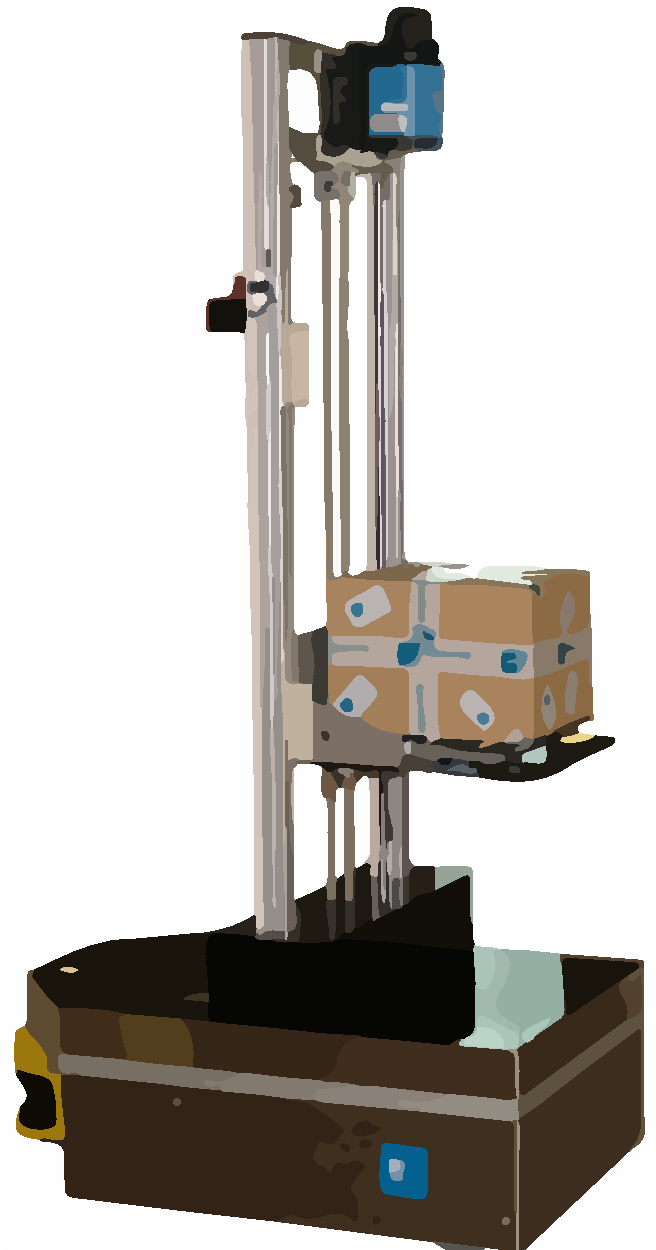
\includegraphics[width=0.28\textwidth]{localization-system-evaluation/testing-platforms/jarvis}
	\caption{Jarvis testing platform}
	\label{fig:localization-system-evaluation_jarvis}
\end{figure}


\subsection{Guardian platform}

The Guardian platform is an autonomous mobile manipulator equipped with a Hokuyo URG-04LX laser in the front and a Hokuyo URG-04LX\_UG01 laser in the back (both mounted about 0.37 meters from the ground). The front laser had a tilting platform which allows 3D mapping of the environment. The arm is a SCHUNK Powerball LWA 4P and in \cref{fig:localization-system-evaluation_guardian} it is attached to a stud welding machine (in simulation it is attached to a video projector). It uses a differential drive locomotion system and can be moved with wheels or with tracks. This platform didn't have a certified ground truth and as such, the results of the performed tests could not be quantified with an external localization system (the results performed with the Gazebo simulator will be presented instead - robot model shown in \cref{fig:localization-system-evaluation_guardian_gazebo}).

\begin{figure}
	\centering
	\begin{minipage}[h]{0.497\textwidth}
		\centering
		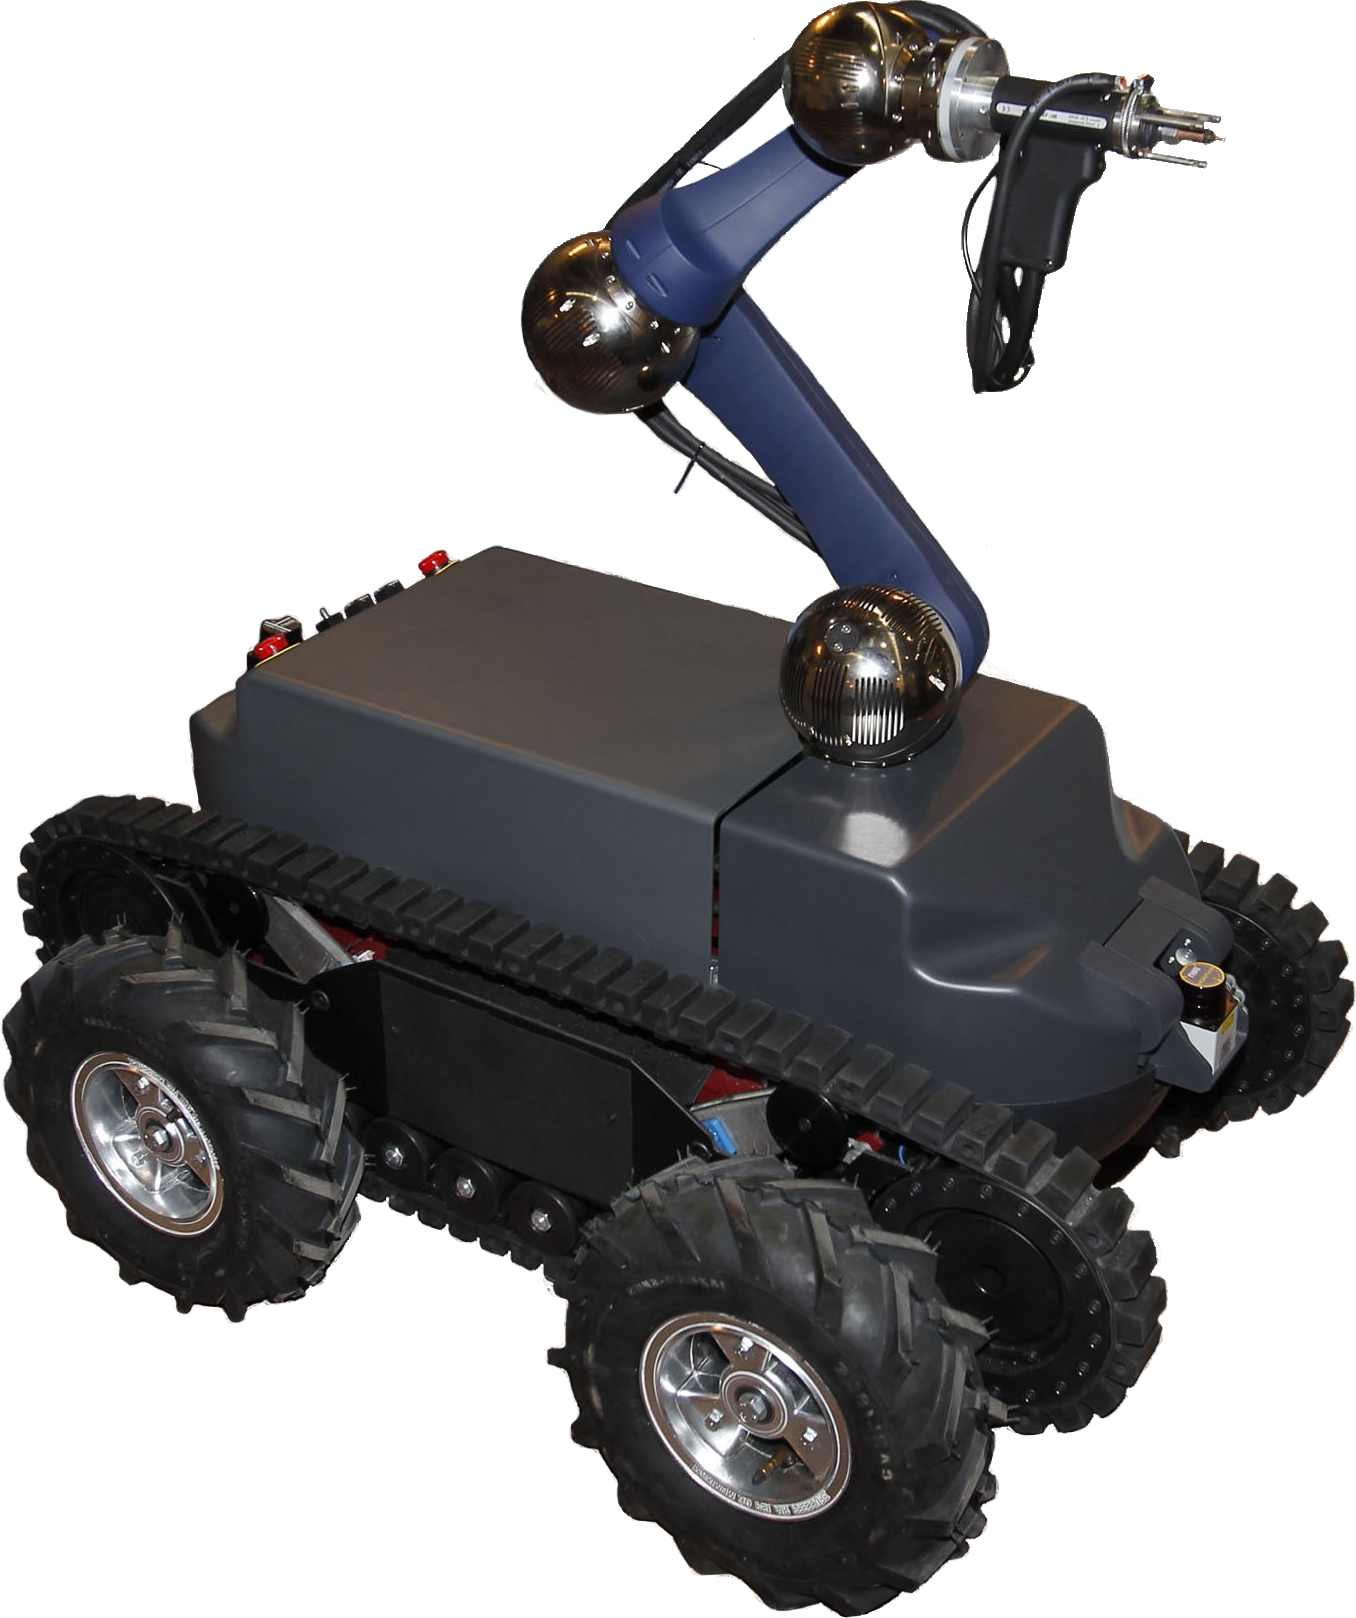
\includegraphics[width=0.67\textwidth]{localization-system-evaluation/testing-platforms/guardian}
		\caption{Guardian testing platform}
		\label{fig:localization-system-evaluation_guardian}
	\end{minipage}\hfill
	\begin{minipage}[h]{0.497\textwidth}
		\centering
		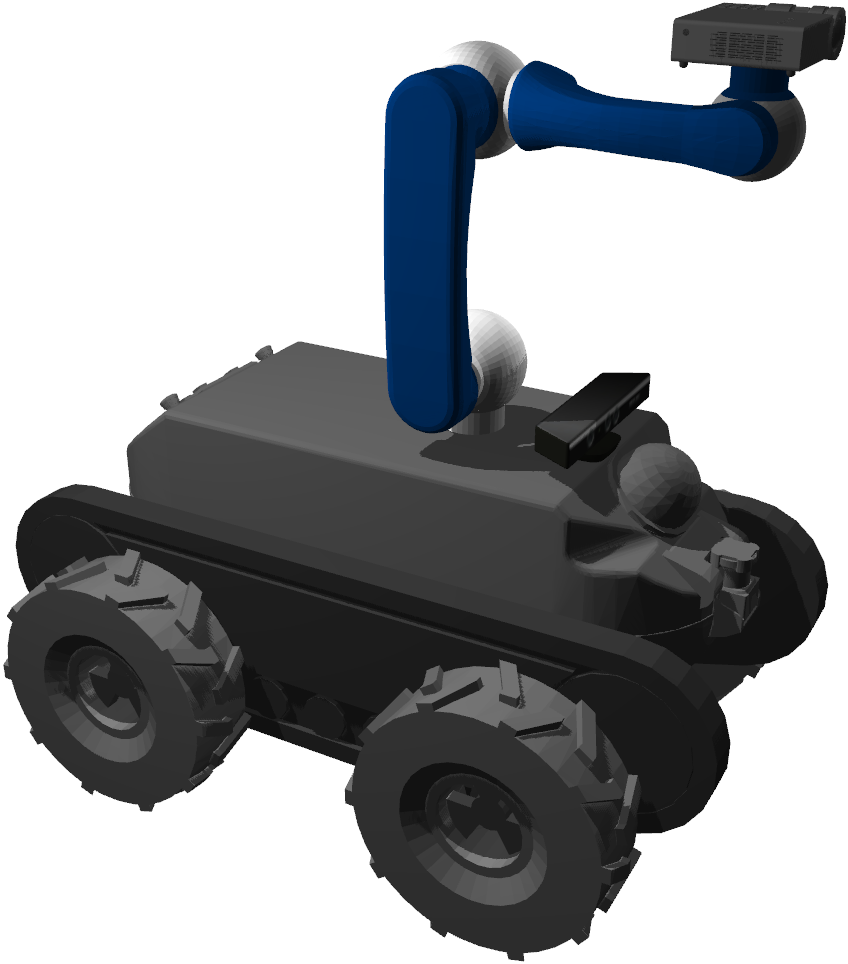
\includegraphics[width=0.67\textwidth]{localization-system-evaluation/testing-platforms/guardian-gazebo}
		\caption{Guardian Gazebo simulation}
		\label{fig:localization-system-evaluation_guardian_gazebo}
	\end{minipage}
\end{figure}


\begin{table}
	\caption{\glsentryplural{lidar} hardware specifications}
	\tabulinesep = 0.9ex
	\centering
	\small
	\begin{tabu} { X[2.5,m,c] | X[m,c] X[m,c] X[m,c] X[m,c] X[m,c] }
		\rowfont{\bfseries\itshape} Laser model & Range (meters) & Field of view (degrees) & Scanning frequency (Hz) & Angular resolution (degrees) & Statistical error (millimeters) \\
		\hline
		{\small SICK NAV350} 			& [0.5..250] 	& 360 	& 8 	& 0.25 	& 15 	\\
		{\small SICK S3000} 			& [0.1..49] 	& 190 	& 8 	& 0.25 	& 150 	\\
		{\small Hokuyo URG-04LX} 		& [0.06..4.095] & 240 	& 10 	& 0.36 	& 10 	\\
		{\small Hokuyo URG-04LX\_UG01} 	& [0.02..4] 	& 240 	& 10 	& 0.36 	& 30 	\\
	\end{tabu}
	\label{tab:localization-system-evaluation_laser-hardware-specifications}
\end{table}


\section{Testing environments}

The localization system was tested using the Jarvis platform in a large room with a RoboCup field and the Guardian platform in a simulated indoor environment with different internal layout variations.


\subsection{Jarvis in RoboCup field}

The RoboCup field (shown in \cref{fig:localization-system-evaluation_jarvis-tests-environment} occupies half of a large room (with 20.5 meters of length and 7.7 meters of depth). It has two doors, several small windows and two large glass openings into the hallway. Several tests were performed with the robot at different speeds in this environment but the ground truth provided by the SICK NAV 350 was only reliable at low paces. As such, only the results of the robot moving at 5 cm/s will be show (along with the tests performed in the Stage simulator\footnote{\url{http://rtv.github.io/Stage/}}). These tests were performed with two different movement paths. The first is a simple rounded path (shown in \cref{fig:localization-system-evaluation_jarvis-robot-circular-path-5cm-per-sec-velocity-1-scan}) that aimed to test the robot in the region of space that had better ground truth (due to its position in relation to the laser reflectors) and the second path was more complex and contained several sub paths with different velocities and shapes (shown in \cref{fig:localization-system-evaluation_jarvis-robot-complex-path-with-outliers-5cm-per-sec-velocity-2-scans}).


\begin{figure}
	\centering
	\begin{subfigure}[h]{.497\textwidth}
		\centering
		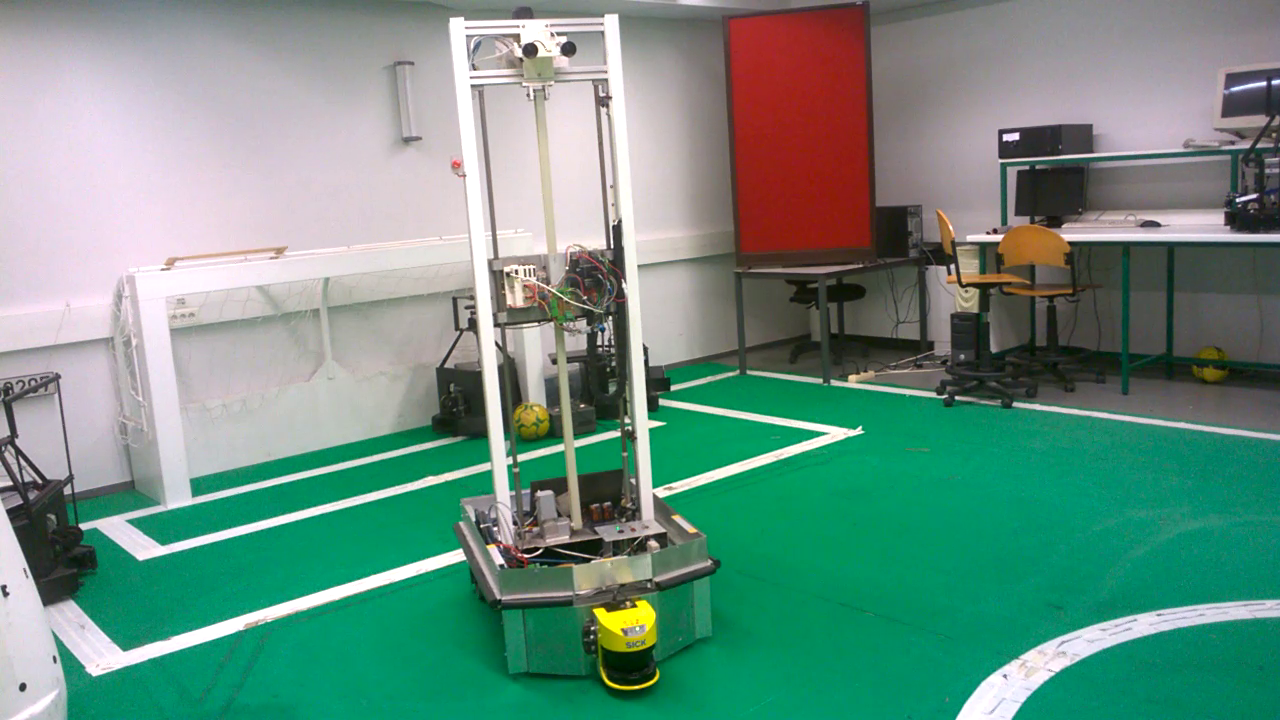
\includegraphics[width=\textwidth]{localization-system-evaluation/testing-environments/jarvis-environment-front-left}
	\end{subfigure}
	\begin{subfigure}[h]{.497\textwidth}
		\centering
		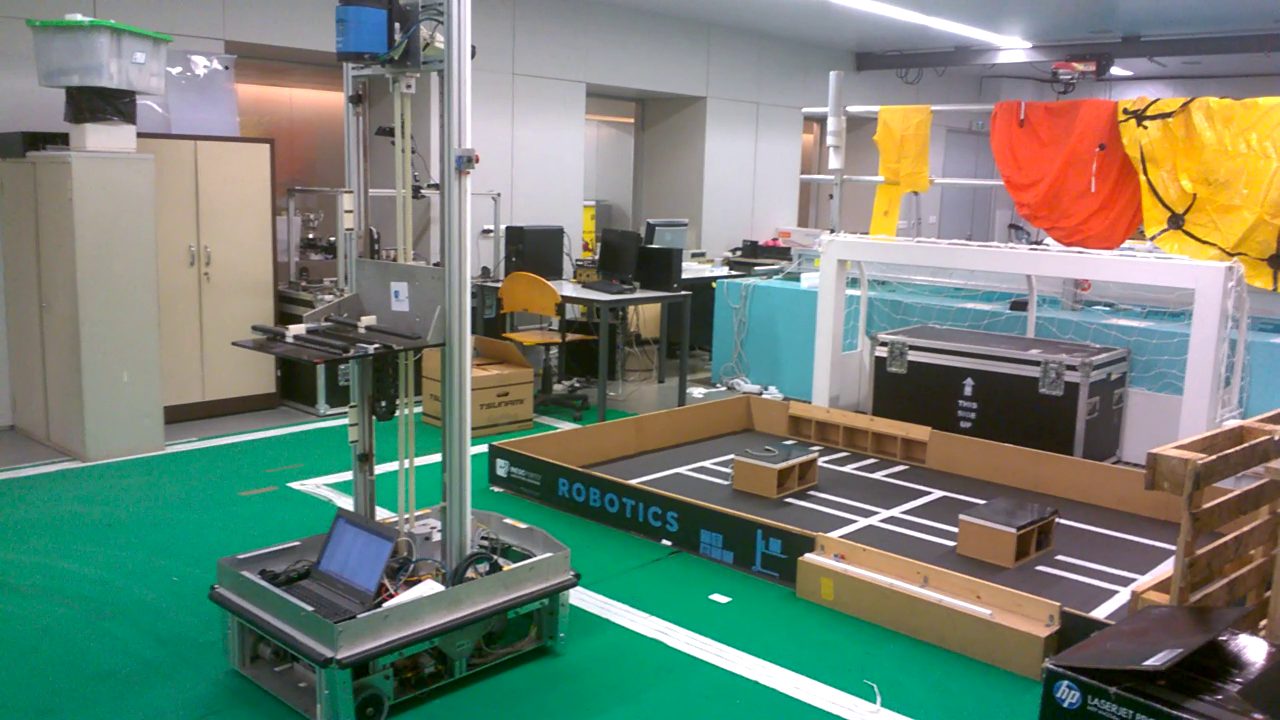
\includegraphics[width=\textwidth]{localization-system-evaluation/testing-environments/jarvis-environment-front-right}
	\end{subfigure}
	\caption{Jarvis tests environment}
	\label{fig:localization-system-evaluation_jarvis-tests-environment}
\end{figure}


\subsection{Guardian in structured environment}

The structured environment simulated in Gazebo is a large room with 12.4 meters of length and 8.4 meters of depth. It has 4 doors, several small windows and the walls have small ledges at regular intervals (as can be seen from \crefrange{fig:localization-system-evaluation_guardian-tests-environment}{fig:localization-system-evaluation_guardian-tests-environment-interactive}).

Given that the Guardian mobile manipulator is expected to work on the walls of this environment, several tests were devised with a path following the lower and right wall of the environment (shown in \cref{fig:localization-system-evaluation_ship-interior-cluttered-dinamic-30cm-per-sec}). The first test was done in a static environment clear of unknown objects and was meant to evaluate the best precision that the localization system could achieve. The second test was done in a cluttered environment and was designed to test the robustness of the localization system against static unknown objects, that were placed in the middle of the environment and close to the walls (to block sensor data from reaching known positions and analyze the robustness of matching unknown points that are close to known areas). The last test added a moving car to the scene and aimed to assess the impact of dynamic objects on the point cloud registration algorithms.


\begin{figure}[H]
	\centering
	\begin{subfigure}[h]{.497\textwidth}
		\centering
		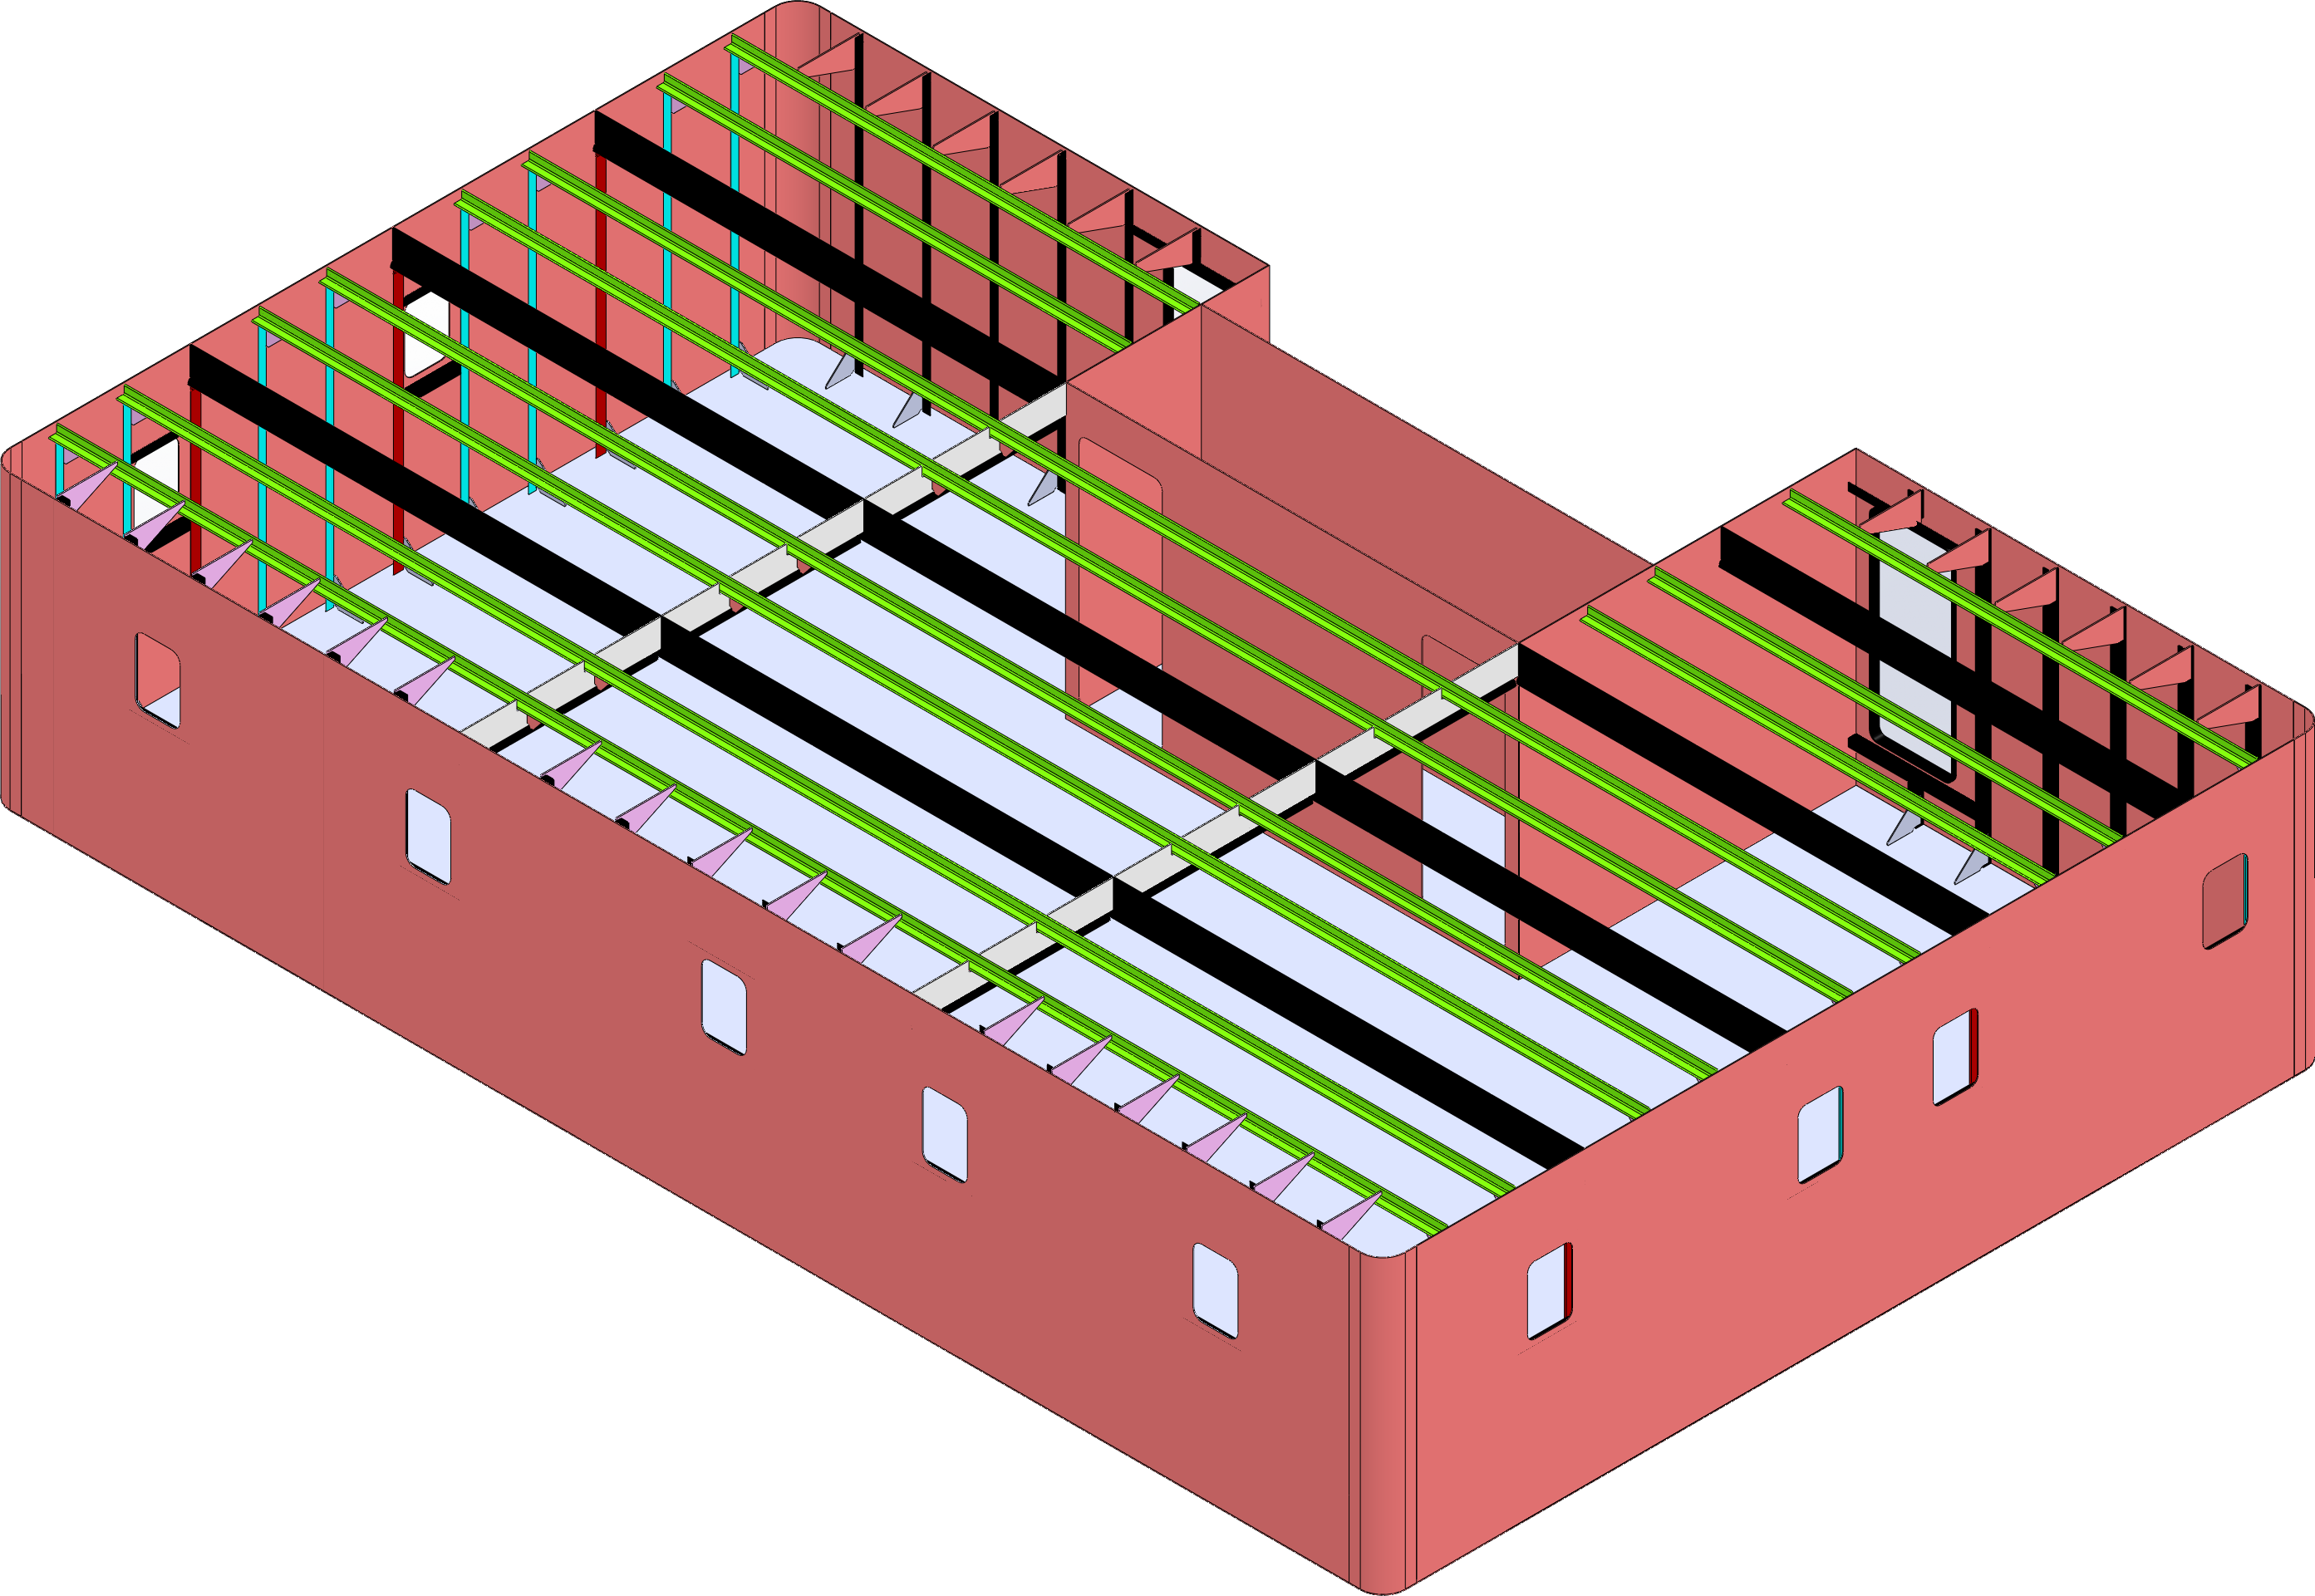
\includegraphics[width=\textwidth]{localization-system-evaluation/testing-environments/guardian-environment-corner}
	\end{subfigure}
	\begin{subfigure}[h]{.497\textwidth}
		\centering
		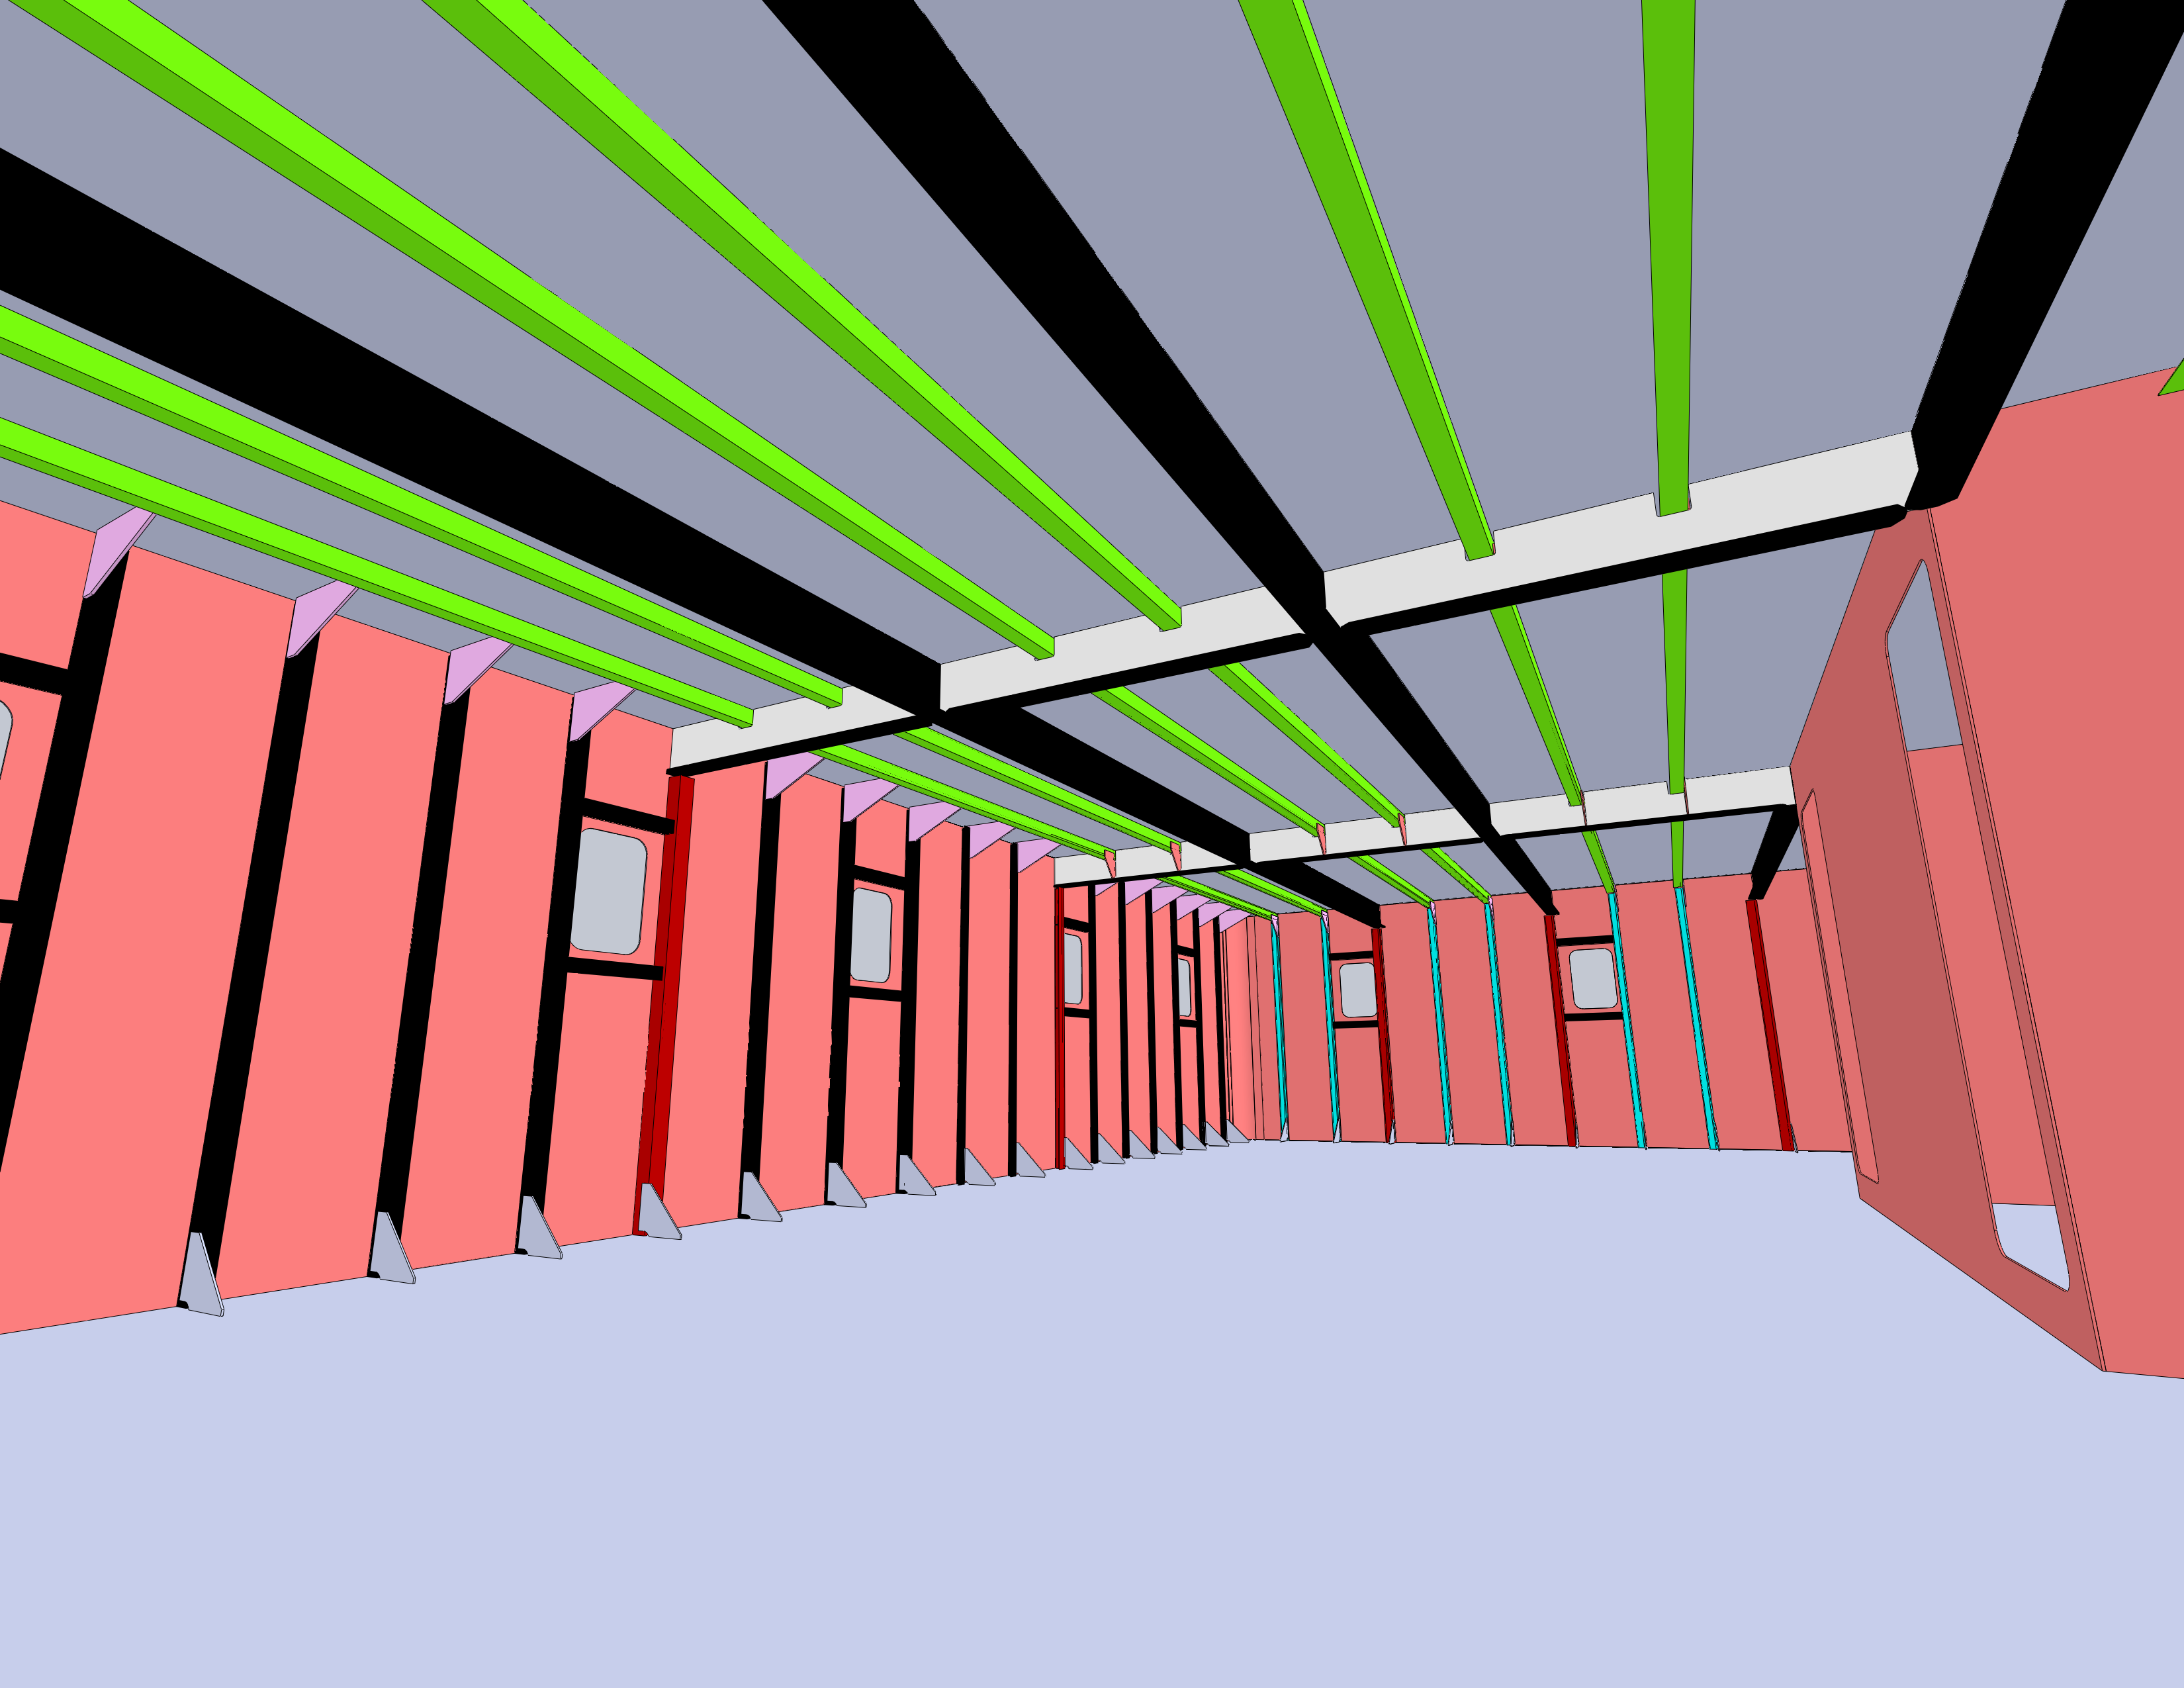
\includegraphics[width=\textwidth]{localization-system-evaluation/testing-environments/guardian-environment-inside}
	\end{subfigure}
	\caption{Guardian testing environment}
	\label{fig:localization-system-evaluation_guardian-tests-environment}
\end{figure}

\begin{figure}[H]
	\centering
	\begin{subfigure}[h]{.497\textwidth}
		\centering
		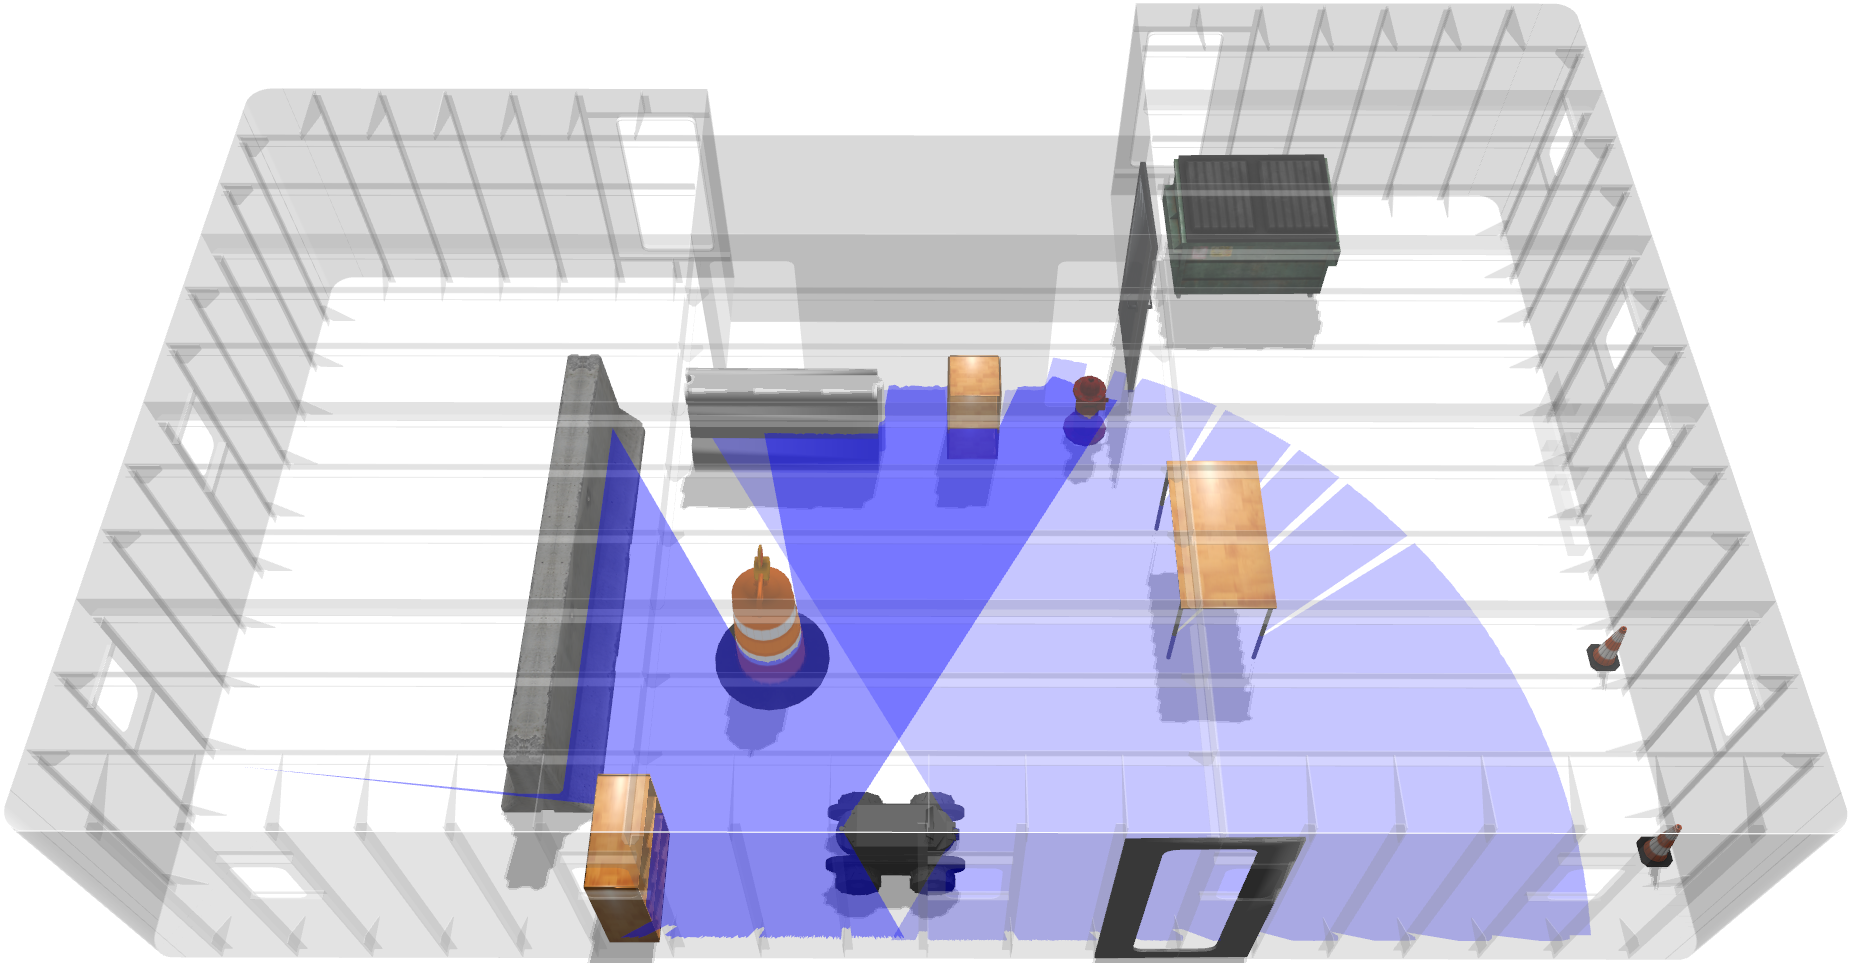
\includegraphics[width=\textwidth]{localization-system-evaluation/testing-environments/guardian-environment-cluttered}
	\end{subfigure}
	\begin{subfigure}[h]{.497\textwidth}
		\centering
		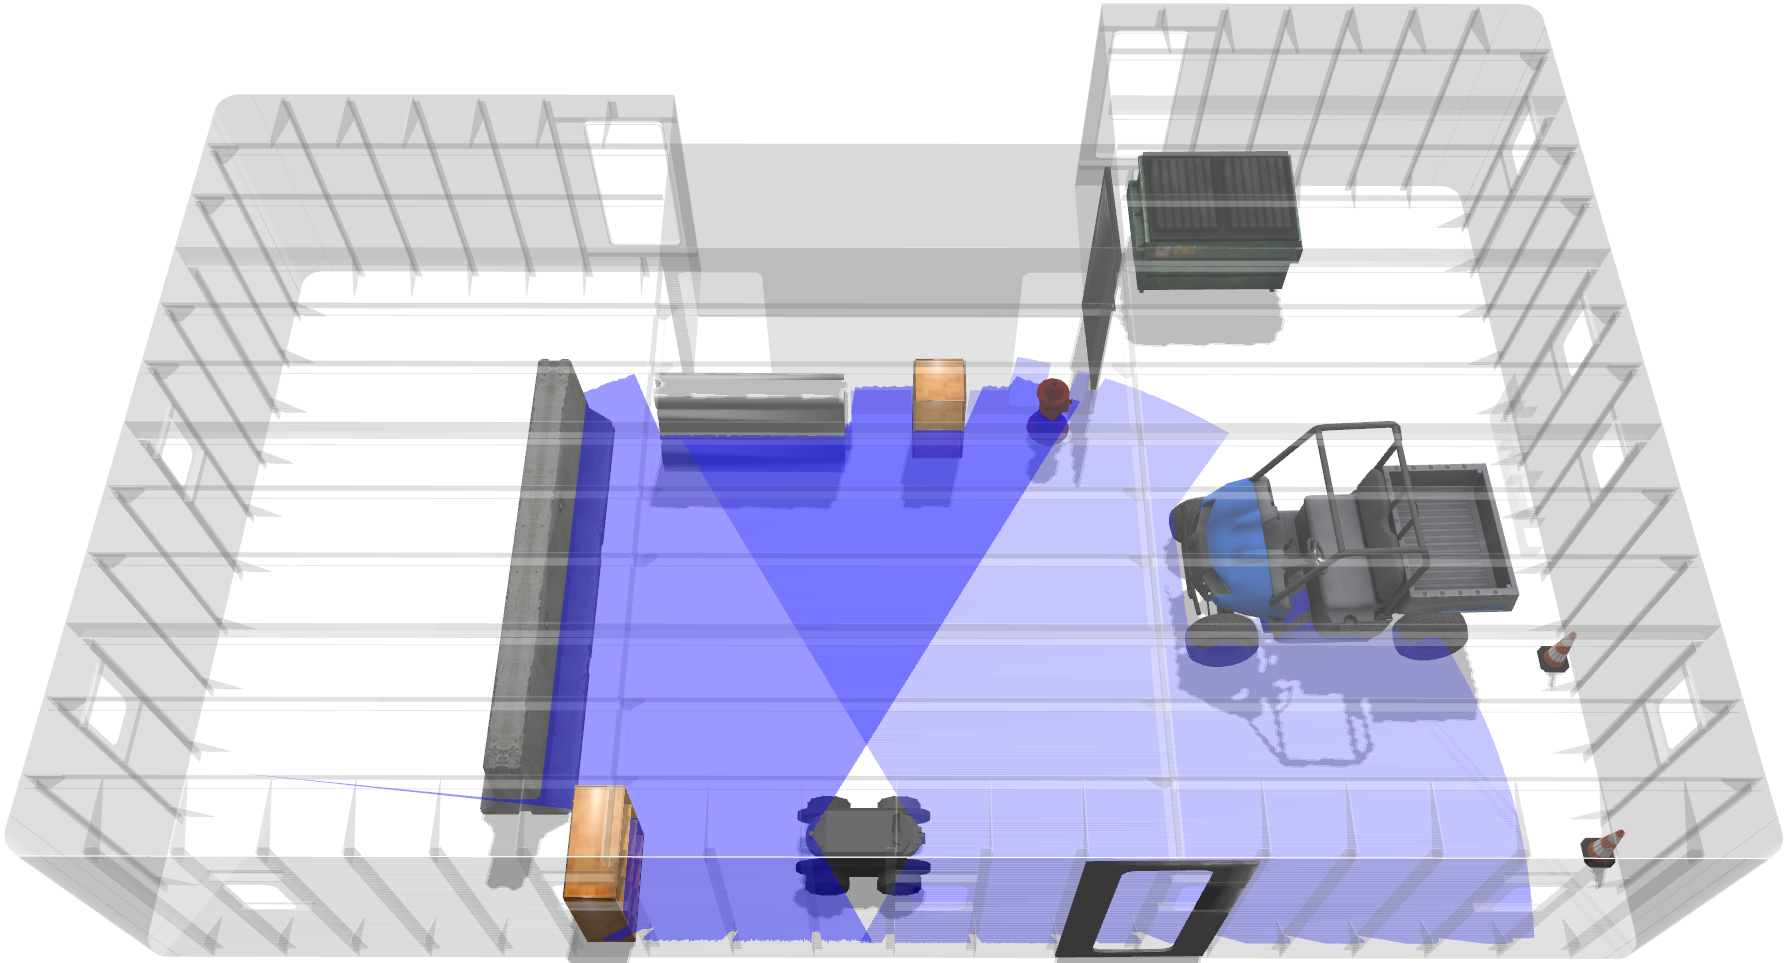
\includegraphics[width=\textwidth]{localization-system-evaluation/testing-environments/guardian-environment-cluttered_dynamic}
	\end{subfigure}
	\caption{Guardian cluttered (left) and dynamic (right) testing environment}
	\label{fig:localization-system-evaluation_guardian-tests-environment-cluttered}
\end{figure}

\begin{figure}[H]
	\centering
	\includemedia[
		label=guardian-environment,
		3Dviews=figures/localization-system-evaluation/testing-environments/guardian-environment.vws,
		width=\linewidth,
		height=0.5\linewidth,
		activate=pageopen,3Dtoolbar,3Dmenu
	]{}{figures/localization-system-evaluation/testing-environments/guardian-environment.u3d}
	\caption{Interactive \glsentrytext{cad} of Guardian testing environment (.u3d file)}
	\label{fig:localization-system-evaluation_guardian-tests-environment-interactive}
\end{figure}



\section{3 \glsentrytext{dof} localization system tests}


\subsection{Overview}

The main results of the 3 \gls{dof} tests performed with the localization system are presented in \cref{tab:localization-system-evaluation_3-dof-results}. It summarizes each test by fitting a normal distribution for each evaluation metric. They were retrieved with a known initial pose using \gls{icp} point-to-point as tracking algorithm and \gls{icp} point-to-plane as tracking recovery method. The Jarvis tests had a map built using the localization system in \gls{slam} mode and were manually corrected to achieve a resolution of 10 mm. The Guardian tests relied on a map built from the \gls{cad} model with resolution of 2 mm. A voxel grid of 75 mm was applied to the assembled laser scans in the Jarvis experiments while in the Guardian tests it was used a voxel grid of 25 mm. The initial pose estimation subsystem used \gls{sift} for keypoint selection, \gls{fpfh} for keypoint description and the feature matching algorithm described in \cref{subsec:localization-system_feature-registration} to estimate the initial position and orientation of the robot (\cref{fig:localization-system-evaluation_ship-interior-initial-pose-estimation-sift-fpfh-ransac-gicp} shows the accepted initial poses when the robot was in the lower right corner of the Guardian test environment).

The next sections contain the main 3 \gls{dof} results of the localization system. To avoid cluttering the next subsections with too many graphs, only the tests with the physical robot platforms will have a detailed analysis (the tests on simulators will only have the movement paths and localization error). In \footnote{\url{https://github.com/carlosmccosta/dynamic_robot_localization_tests}} is available the full test results along with videos and the configurations used.

The robot movement paths present in the next sections illustrate the synchronized poses from the localization system (blue arrows), ground truth (green arrows) and odometry (red arrows). A regular grid with one meter spacing was applied on top of the figures to ease their analysis.


\begin{sidewaystable}
	\caption{3 \glsentrytext{dof} localization system results}
	\tabulinesep = 1.2ex
%	\setlength{\tabcolsep}{0.2em}
	\centering
	\tiny
	\begin{tabu} to \textwidth { X[m,c] X[m,c] X[m,c] X[1.5m,c] X[m,c] X[0.01m,c] X[m,c] X[m,c] X[0.01m,c] X[m,c] X[m,c] X[0.01m,c] X[m,c] X[m,c] X[0.01m,c] X[m,c] X[m,c] }
		\hline
		\multicolumn{5}{c}{Test conditions} && \multicolumn{2}{c}{Translation error (millimeters)} && \multicolumn{2}{c}{Rotation error (degrees)} && \multicolumn{2}{c}{Outliers percentage [0..100]} && \multicolumn{2}{c}{Global computation time (milliseconds)} \\
		\cline{1-5} \cline{7-8} \cline{10-11} \cline{13-14} \cline{16-17}
		Platform 																& Ambient 													& Path shape 											& Path velocities 		& Nº scans / Nº lasers 			&& Mean  & Standard deviation 	&& Mean  & Standard deviation 	&& Mean  & Standard deviation 	&& Mean   & Standard deviation \\ \hline
		\multirow{2}{0.05\textwidth}{\centering Jarvis robot} 					& Cluttered 												& Rounded 												& 5 cm/s 				& 1/1 							&& 5.608 & 3.280 				&& 0.634 & 0.169 				&& 12.21 & 4.50 				&& 7.065  & 6.456 	\\ \tabucline[0.5pt on 3pt off 2pt]{2-3}
																				& Cluttered dynamic 										& Complex 												& 5 cm/s 				& 2/1 							&& 6.235 & 3.242 				&& 0.529 & 0.157 				&& 20.16 & 5.87 				&& 7.827  & 7.990 	\\ \tabucline[0.5pt on 3pt off 2pt]{1-3}
		\multirow{6}{0.05\textwidth}{\centering Jarvis simulator (Stage)} 		& \multirow{6}{0.05\textwidth}{\centering Cluttered} 		& \multirow{3}{0.05\textwidth}{\centering Rounded} 		& 5 cm/s 				& 2/1 							&& 2.817 & 1.551 				&& 0.038 & 0.026 				&& 16.11 & 0.93 				&& 12.600 & 12.459 	\\
																				&  															&  														& 50 cm/s 				& 2/1 							&& 4.479 & 3.769 				&& 0.106 & 0.137 				&& 15.82 & 1.14 				&& 24.500 & 13.592 	\\
																				&  															&  														& 100 cm/s 				& 1/1 							&& 4.710 & 2.788 				&& 0.135 & 0.134 				&& 16.13 & 0.92 				&& 16.432 & 12.291 	\\ \tabucline[0.5pt on 3pt off 2pt]{3-3}
																				&  															& \multirow{3}{0.05\textwidth}{\centering Complex} 		& 5 cm/s 				& 2/1 							&& 2.476 & 1.370 				&& 0.017 & 0.017 				&& 17.00 & 0.92 				&& 10.374 & 12.138 	\\
																				&  															&  														& 50-30-50-20 cm/s 		& 2/1 							&& 3.557 & 1.800 				&& 0.033 & 0.040 				&& 17.61 & 1.33 				&& 14.863 & 15.898 	\\
																				&  															&  														& 200-30-200-30 cm/s 	& 2/1 							&& 4.199 & 2.596 				&& 0.048 & 0.110 				&& 17.84 & 1.23 				&& 13.150 & 14.351 	\\ \tabucline[0.5pt on 3pt off 2pt]{1-3}
		\multirow{6}{0.05\textwidth}{\centering Guardian simulator (Gazebo)} 	& \multirow{2}{0.05\textwidth}{\centering Static} 			& \multirow{6}{0.05\textwidth}{\centering Wall follower}& 5 cm/s 				& 2/2 							&& 2.642 & 0.463 				&& 0.016 & 0.023 				&& 0.0   & 0.0  				&& 5.723  & 1.868 	\\
																				&  															&  														& 30 cm/s 				& 2/2 							&& 4.961 & 3.953 				&& 0.032 & 0.084 				&& 0.0   & 0.0  				&& 6.365  & 2.906 	\\ \tabucline[0.5pt on 3pt off 2pt]{2-2}
																				& \multirow{2}{0.05\textwidth}{\centering Cluttered} 		&  														& 5 cm/s 				& 2/2 							&& 2.912 & 0.856 				&& 0.020 & 0.026 				&& 25.05 & 13.30 				&& 11.889 & 9.084 	\\
																				&  															& 														& 30 cm/s 				& 2/2 							&& 6.713 & 6.380 				&& 0.141 & 0.203 				&& 30.39 & 14.66 				&& 25.367 & 35.724 	\\ \tabucline[0.5pt on 3pt off 2pt]{2-2}
																				& \multirow{2}{0.05\textwidth}{\centering Cluttered dynamic}&  														& 5 cm/s 				& 2/2 							&& 4.593 & 3.802 				&& 0.069 & 0.072 				&& 33.33 & 9.88  				&& 22.217 & 32.408 	\\
																				&  															&  														& 30 cm/s 				& 2/2 							&& 5.847 & 5.585 				&& 0.105 & 0.125 				&& 34.20 & 16.64 				&& 26.892 & 35.630 	\\
		\hline
	\end{tabu}
	\label{tab:localization-system-evaluation_3-dof-results}
\end{sidewaystable}


\clearpage
\subsection{Jarvis robot tests}

\subsubsection{Rounded path using Jarvis robot at 5 cm/s}

\Crefrange{fig:localization-system-evaluation_jarvis-robot-circular-path-5cm-per-sec-velocity-1-scan}{fig:localization-system-evaluation_jarvis-robot-circular-path-5cm-per-sec-velocity-1-scan_computation-time} show the detailed results of the Jarvis robot in the RoboCup field following a rounded path and moving at 5 cm/s.

\begin{figure}[H]
	\centering
	\includegraphics[width=\textwidth]{localization-system-evaluation/tests-3dof/jarvis-robot-circular-path-5cm-per-sec-velocity-1-scan/robot-movement-path-with-odometry-and-map}
	\caption{Paths from ground truth (green), localization system (blue) and odometry (red)}
	\label{fig:localization-system-evaluation_jarvis-robot-circular-path-5cm-per-sec-velocity-1-scan}
\end{figure}

\begin{figure}[H]
	\centering
	\begin{subfigure}[h]{.497\textwidth}
		\centering
		\includegraphics[width=\textwidth]{localization-system-evaluation/tests-3dof/jarvis-robot-circular-path-5cm-per-sec-velocity-1-scan/translation-error-millimeters}
	\end{subfigure}
	\begin{subfigure}[h]{.497\textwidth}
		\centering
		\includegraphics[width=\textwidth]{localization-system-evaluation/tests-3dof/jarvis-robot-circular-path-5cm-per-sec-velocity-1-scan/translation-error-millimeters-distributions}
	\end{subfigure}
	\caption{Localization system translation error (left) and its statistical distributions (right)}
	\label{fig:localization-system-evaluation_jarvis-robot-circular-path-5cm-per-sec-velocity-1-scan_translation-errors}
\end{figure}

\begin{figure}[H]
	\centering
	\begin{subfigure}[h]{.497\textwidth}
		\centering
		\includegraphics[width=\textwidth]{localization-system-evaluation/tests-3dof/jarvis-robot-circular-path-5cm-per-sec-velocity-1-scan/translation-correction-millimeters}
	\end{subfigure}
	\begin{subfigure}[h]{.497\textwidth}
		\centering
		\includegraphics[width=\textwidth]{localization-system-evaluation/tests-3dof/jarvis-robot-circular-path-5cm-per-sec-velocity-1-scan/translation-correction-millimeters-distributions}
	\end{subfigure}
	\caption{Localization system translation corrections (left) and its statistical distributions (right)}
	\label{fig:localization-system-evaluation_jarvis-robot-circular-path-5cm-per-sec-velocity-1-scan_translation-errors-corrections}
\end{figure}

\begin{figure}[ht]
	\centering
	\begin{subfigure}[h]{.497\textwidth}
		\centering
		\includegraphics[width=\textwidth]{localization-system-evaluation/tests-3dof/jarvis-robot-circular-path-5cm-per-sec-velocity-1-scan/translation-error-components-millimeters}
	\end{subfigure}
	\begin{subfigure}[h]{.497\textwidth}
		\centering
		\includegraphics[width=\textwidth]{localization-system-evaluation/tests-3dof/jarvis-robot-circular-path-5cm-per-sec-velocity-1-scan/translation-corrections-components-millimeters}
	\end{subfigure}
	\caption{Localization system translation error (left) and corrections (right) components}
	\label{fig:localization-system-evaluation_jarvis-robot-circular-path-5cm-per-sec-velocity-1-scan_translation-errors-components}
\end{figure}

\begin{figure}[ht]
	\centering
	\begin{subfigure}[h]{.497\textwidth}
		\centering
		\includegraphics[width=\textwidth]{localization-system-evaluation/tests-3dof/jarvis-robot-circular-path-5cm-per-sec-velocity-1-scan/rotation-error-degrees}
	\end{subfigure}
	\begin{subfigure}[h]{.497\textwidth}
		\centering
		\includegraphics[width=\textwidth]{localization-system-evaluation/tests-3dof/jarvis-robot-circular-path-5cm-per-sec-velocity-1-scan/rotation-error-degrees-distributions}
	\end{subfigure}
	\caption{Localization system rotation error (left) and its statistical distributions (right)}
	\label{fig:localization-system-evaluation_jarvis-robot-circular-path-5cm-per-sec-velocity-1-scan_rotation-errors}
\end{figure}

\begin{figure}[ht]
	\centering
	\begin{subfigure}[h]{.497\textwidth}
		\centering
		\includegraphics[width=\textwidth]{localization-system-evaluation/tests-3dof/jarvis-robot-circular-path-5cm-per-sec-velocity-1-scan/rotation-correction-degrees}
	\end{subfigure}
	\begin{subfigure}[h]{.497\textwidth}
		\centering
		\includegraphics[width=\textwidth]{localization-system-evaluation/tests-3dof/jarvis-robot-circular-path-5cm-per-sec-velocity-1-scan/rotation-correction-degrees-distributions}
	\end{subfigure}
	\caption{Localization system rotation corrections (left) and its statistical distributions (right)}
	\label{fig:localization-system-evaluation_jarvis-robot-circular-path-5cm-per-sec-velocity-1-scan_rotation-errors-corrections}
\end{figure}

\begin{figure}[ht]
	\centering
	\begin{subfigure}[h]{.497\textwidth}
		\centering
		\includegraphics[width=\textwidth]{localization-system-evaluation/tests-3dof/jarvis-robot-circular-path-5cm-per-sec-velocity-1-scan/odometry-translation-error-millimeters}
	\end{subfigure}
	\begin{subfigure}[h]{.497\textwidth}
		\centering
		\includegraphics[width=\textwidth]{localization-system-evaluation/tests-3dof/jarvis-robot-circular-path-5cm-per-sec-velocity-1-scan/odometry-translation-error-millimeters-distributions}
	\end{subfigure}
	\caption{Odometry translation error (left) and its statistical distributions (right)}
	\label{fig:localization-system-evaluation_jarvis-robot-circular-path-5cm-per-sec-velocity-1-scan_odometry-translation-errors}
\end{figure}

\begin{figure}[ht]
	\centering
	\begin{subfigure}[h]{.497\textwidth}
		\centering
		\includegraphics[width=\textwidth]{localization-system-evaluation/tests-3dof/jarvis-robot-circular-path-5cm-per-sec-velocity-1-scan/odometry-rotation-error-degrees}
	\end{subfigure}
	\begin{subfigure}[h]{.497\textwidth}
		\centering
		\includegraphics[width=\textwidth]{localization-system-evaluation/tests-3dof/jarvis-robot-circular-path-5cm-per-sec-velocity-1-scan/odometry-rotation-error-degrees-distributions}
	\end{subfigure}
	\caption{Odometry rotation error (left) and its statistical distributions (right)}
	\label{fig:localization-system-evaluation_jarvis-robot-circular-path-5cm-per-sec-velocity-1-scan_odometry-rotation-errors}
\end{figure}

\begin{figure}[ht]
	\centering
	\begin{subfigure}[h]{.497\textwidth}
		\centering
		\includegraphics[width=\textwidth]{localization-system-evaluation/tests-3dof/jarvis-robot-circular-path-5cm-per-sec-velocity-1-scan/root-mean-square-error-inliers}
	\end{subfigure}
	\begin{subfigure}[h]{.497\textwidth}
		\centering
		\includegraphics[width=\textwidth]{localization-system-evaluation/tests-3dof/jarvis-robot-circular-path-5cm-per-sec-velocity-1-scan/root-mean-square-error-inliers-distributions}
	\end{subfigure}
	\caption{Localization system inliers \glsentrytext{rmse} (left) and its statistical distributions (right)}
	\label{fig:localization-system-evaluation_jarvis-robot-circular-path-5cm-per-sec-velocity-1-scan_inliers-rmse}
\end{figure}

\begin{figure}[ht]
	\centering
	\begin{subfigure}[h]{.497\textwidth}
		\centering
		\includegraphics[width=\textwidth]{localization-system-evaluation/tests-3dof/jarvis-robot-circular-path-5cm-per-sec-velocity-1-scan/outlier-percentage}
	\end{subfigure}
	\begin{subfigure}[h]{.497\textwidth}
		\centering
		\includegraphics[width=\textwidth]{localization-system-evaluation/tests-3dof/jarvis-robot-circular-path-5cm-per-sec-velocity-1-scan/registered-points-angular-distribution}
	\end{subfigure}
	\caption{Cloud registration outlier percentage (left) and inliers angular distribution (right)}
	\label{fig:localization-system-evaluation_jarvis-robot-circular-path-5cm-per-sec-velocity-1-scan_analysis}
\end{figure}

\begin{figure}[ht]
	\centering
	\includegraphics[width=0.5\textwidth]{localization-system-evaluation/tests-3dof/jarvis-robot-circular-path-5cm-per-sec-velocity-1-scan/computation-times-milliseconds}
	\caption{Localization system computation times}
	\label{fig:localization-system-evaluation_jarvis-robot-circular-path-5cm-per-sec-velocity-1-scan_computation-time}
\end{figure}

\clearpage
\subsubsection{Complex path using Jarvis robot at 5 cm/s}

\Crefrange{fig:localization-system-evaluation_jarvis-robot-complex-path-with-outliers-5cm-per-sec-velocity-2-scans}{fig:localization-system-evaluation_jarvis-robot-complex-path-with-outliers-5cm-per-sec-velocity-2-scans_computation-time} show the detailed results of the Jarvis robot in the RoboCup field following a complex path and moving at 5 cm/s.

\begin{figure}[H]
	\centering
	\includegraphics[width=\textwidth]{localization-system-evaluation/tests-3dof/jarvis-robot-complex-path-with-outliers-5cm-per-sec-velocity-2-scans/robot-movement-path-with-odometry-and-map}
	\caption{Paths from ground truth (green), localization system (blue) and odometry (red)}
	\label{fig:localization-system-evaluation_jarvis-robot-complex-path-with-outliers-5cm-per-sec-velocity-2-scans}
\end{figure}

\begin{figure}[H]
	\centering
	\begin{subfigure}[h]{.497\textwidth}
		\centering
		\includegraphics[width=\textwidth]{localization-system-evaluation/tests-3dof/jarvis-robot-complex-path-with-outliers-5cm-per-sec-velocity-2-scans/translation-error-millimeters}
	\end{subfigure}
	\begin{subfigure}[h]{.497\textwidth}
		\centering
		\includegraphics[width=\textwidth]{localization-system-evaluation/tests-3dof/jarvis-robot-complex-path-with-outliers-5cm-per-sec-velocity-2-scans/translation-error-millimeters-distributions}
	\end{subfigure}
	\caption{Localization system translation error (left) and its statistical distributions (right)}
	\label{fig:localization-system-evaluation_jarvis-robot-complex-path-with-outliers-5cm-per-sec-velocity-2-scans_translation-errors}
\end{figure}

\begin{figure}[H]
	\centering
	\begin{subfigure}[h]{.497\textwidth}
		\centering
		\includegraphics[width=\textwidth]{localization-system-evaluation/tests-3dof/jarvis-robot-complex-path-with-outliers-5cm-per-sec-velocity-2-scans/translation-correction-millimeters}
	\end{subfigure}
	\begin{subfigure}[h]{.497\textwidth}
		\centering
		\includegraphics[width=\textwidth]{localization-system-evaluation/tests-3dof/jarvis-robot-complex-path-with-outliers-5cm-per-sec-velocity-2-scans/translation-correction-millimeters-distributions}
	\end{subfigure}
	\caption{Localization system translation corrections (left) and its statistical distributions (right)}
	\label{fig:localization-system-evaluation_jarvis-robot-complex-path-with-outliers-5cm-per-sec-velocity-2-scans_translation-errors-corrections}
\end{figure}

\begin{figure}[ht]
	\centering
	\begin{subfigure}[h]{.497\textwidth}
		\centering
		\includegraphics[width=\textwidth]{localization-system-evaluation/tests-3dof/jarvis-robot-complex-path-with-outliers-5cm-per-sec-velocity-2-scans/translation-error-components-millimeters}
	\end{subfigure}
	\begin{subfigure}[h]{.497\textwidth}
		\centering
		\includegraphics[width=\textwidth]{localization-system-evaluation/tests-3dof/jarvis-robot-complex-path-with-outliers-5cm-per-sec-velocity-2-scans/translation-corrections-components-millimeters}
	\end{subfigure}
	\caption{Localization system translation error (left) and corrections (right) components}
	\label{fig:localization-system-evaluation_jarvis-robot-complex-path-with-outliers-5cm-per-sec-velocity-2-scans_translation-errors-components}
\end{figure}

\begin{figure}[ht]
	\centering
	\begin{subfigure}[h]{.497\textwidth}
		\centering
		\includegraphics[width=\textwidth]{localization-system-evaluation/tests-3dof/jarvis-robot-complex-path-with-outliers-5cm-per-sec-velocity-2-scans/rotation-error-degrees}
	\end{subfigure}
	\begin{subfigure}[h]{.497\textwidth}
		\centering
		\includegraphics[width=\textwidth]{localization-system-evaluation/tests-3dof/jarvis-robot-complex-path-with-outliers-5cm-per-sec-velocity-2-scans/rotation-error-degrees-distributions}
	\end{subfigure}
	\caption{Localization system rotation error (left) and its statistical distributions (right)}
	\label{fig:localization-system-evaluation_jarvis-robot-complex-path-with-outliers-5cm-per-sec-velocity-2-scans_rotation-errors}
\end{figure}

\begin{figure}[ht]
	\centering
	\begin{subfigure}[h]{.497\textwidth}
		\centering
		\includegraphics[width=\textwidth]{localization-system-evaluation/tests-3dof/jarvis-robot-complex-path-with-outliers-5cm-per-sec-velocity-2-scans/rotation-correction-degrees}
	\end{subfigure}
	\begin{subfigure}[h]{.497\textwidth}
		\centering
		\includegraphics[width=\textwidth]{localization-system-evaluation/tests-3dof/jarvis-robot-complex-path-with-outliers-5cm-per-sec-velocity-2-scans/rotation-correction-degrees-distributions}
	\end{subfigure}
	\caption{Localization system rotation corrections (left) and its statistical distributions (right)}
	\label{fig:localization-system-evaluation_jarvis-robot-complex-path-with-outliers-5cm-per-sec-velocity-2-scans_rotation-errors-corrections}
\end{figure}

\begin{figure}[ht]
	\centering
	\begin{subfigure}[h]{.497\textwidth}
		\centering
		\includegraphics[width=\textwidth]{localization-system-evaluation/tests-3dof/jarvis-robot-complex-path-with-outliers-5cm-per-sec-velocity-2-scans/odometry-translation-error-millimeters}
	\end{subfigure}
	\begin{subfigure}[h]{.497\textwidth}
		\centering
		\includegraphics[width=\textwidth]{localization-system-evaluation/tests-3dof/jarvis-robot-complex-path-with-outliers-5cm-per-sec-velocity-2-scans/odometry-translation-error-millimeters-distributions}
	\end{subfigure}
	\caption{Odometry translation error (left) and its statistical distributions (right)}
	\label{fig:localization-system-evaluation_jarvis-robot-complex-path-with-outliers-5cm-per-sec-velocity-2-scans_odometry-translation-errors}
\end{figure}

\begin{figure}[ht]
	\centering
	\begin{subfigure}[h]{.497\textwidth}
		\centering
		\includegraphics[width=\textwidth]{localization-system-evaluation/tests-3dof/jarvis-robot-complex-path-with-outliers-5cm-per-sec-velocity-2-scans/odometry-rotation-error-degrees}
	\end{subfigure}
	\begin{subfigure}[h]{.497\textwidth}
		\centering
		\includegraphics[width=\textwidth]{localization-system-evaluation/tests-3dof/jarvis-robot-complex-path-with-outliers-5cm-per-sec-velocity-2-scans/odometry-rotation-error-degrees-distributions}
	\end{subfigure}
	\caption{Odometry rotation error (left) and its statistical distributions (right)}
	\label{fig:localization-system-evaluation_jarvis-robot-complex-path-with-outliers-5cm-per-sec-velocity-2-scans_odometry-rotation-errors}
\end{figure}

\begin{figure}[ht]
	\centering
	\begin{subfigure}[h]{.497\textwidth}
		\centering
		\includegraphics[width=\textwidth]{localization-system-evaluation/tests-3dof/jarvis-robot-complex-path-with-outliers-5cm-per-sec-velocity-2-scans/root-mean-square-error-inliers}
	\end{subfigure}
	\begin{subfigure}[h]{.497\textwidth}
		\centering
		\includegraphics[width=\textwidth]{localization-system-evaluation/tests-3dof/jarvis-robot-complex-path-with-outliers-5cm-per-sec-velocity-2-scans/root-mean-square-error-inliers-distributions}
	\end{subfigure}
	\caption{Localization system inliers \glsentrytext{rmse} (left) and its statistical distributions (right)}
	\label{fig:localization-system-evaluation_jarvis-robot-complex-path-with-outliers-5cm-per-sec-velocity-2-scans_inliers-rmse}
\end{figure}

\begin{figure}[ht]
	\centering
	\begin{subfigure}[h]{.497\textwidth}
		\centering
		\includegraphics[width=\textwidth]{localization-system-evaluation/tests-3dof/jarvis-robot-complex-path-with-outliers-5cm-per-sec-velocity-2-scans/outlier-percentage}
	\end{subfigure}
	\begin{subfigure}[h]{.497\textwidth}
		\centering
		\includegraphics[width=\textwidth]{localization-system-evaluation/tests-3dof/jarvis-robot-complex-path-with-outliers-5cm-per-sec-velocity-2-scans/registered-points-angular-distribution}
	\end{subfigure}
	\caption{Cloud registration outlier percentage (left) and inliers angular distribution (right)}
	\label{fig:localization-system-evaluation_jarvis-robot-complex-path-with-outliers-5cm-per-sec-velocity-2-scans_analysis}
\end{figure}

\begin{figure}[ht]
	\centering
	\includegraphics[width=0.5\textwidth]{localization-system-evaluation/tests-3dof/jarvis-robot-complex-path-with-outliers-5cm-per-sec-velocity-2-scans/computation-times-milliseconds}
	\caption{Localization system computation times}
	\label{fig:localization-system-evaluation_jarvis-robot-complex-path-with-outliers-5cm-per-sec-velocity-2-scans_computation-time}
\end{figure}

\clearpage

\subsection{Jarvis simulator tests}


\subsubsection{Rounded path using Jarvis simulator at 5 cm/s}

\Crefrange{fig:localization-system-evaluation_jarvis-simulator-circular-path-5cm-per-sec-velocity-2-scans}{fig:localization-system-evaluation_jarvis-simulator-circular-path-5cm-per-sec-velocity-2-scans_angular-distribution-analysis-computation-time} show the results of the Jarvis platform using the Stage simulator in the RoboCup field map following a rounded path and moving at 5 cm/s.

\begin{figure}[H]
	\centering
	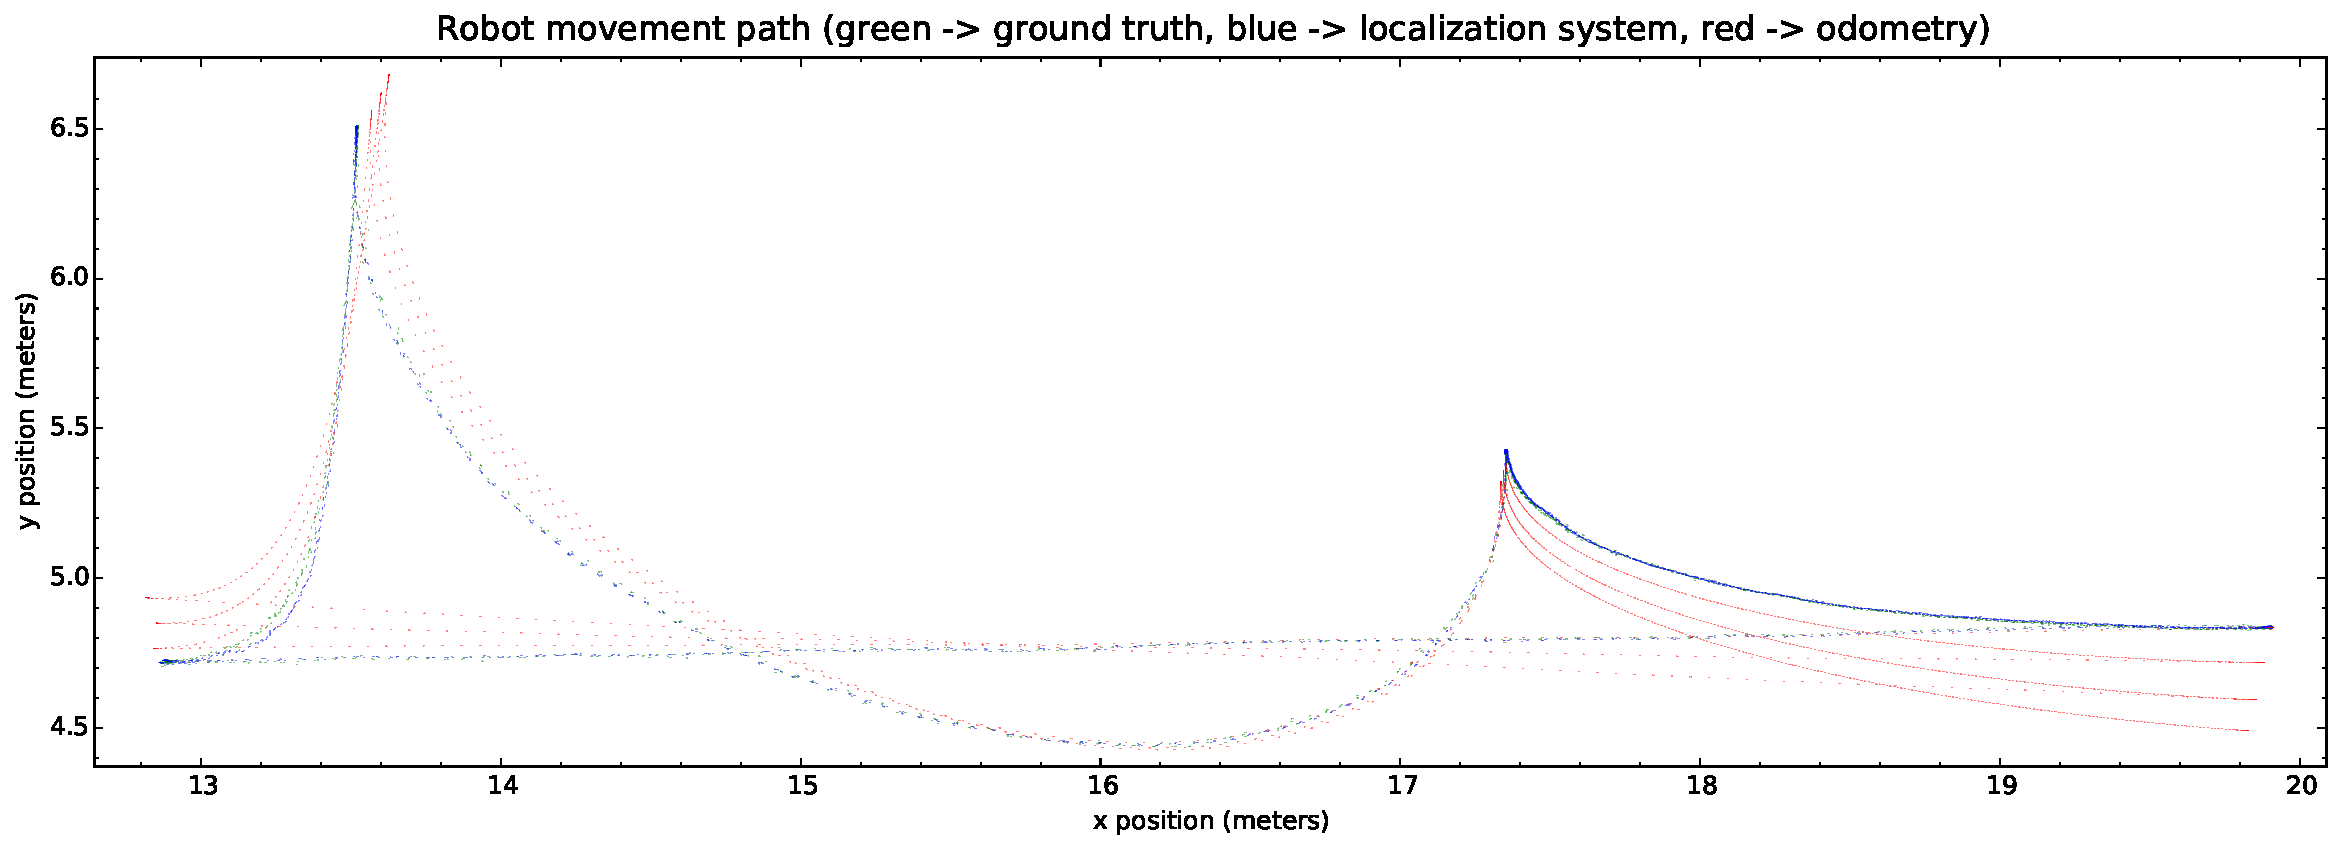
\includegraphics[width=0.5\textwidth]{localization-system-evaluation/tests-3dof/jarvis-simulator-circular-path-5cm-per-sec-velocity-2-scans/robot-movement-path-with-odometry}
	\caption{Paths from ground truth (green), localization system (blue) and odometry (red)}
	\label{fig:localization-system-evaluation_jarvis-simulator-circular-path-5cm-per-sec-velocity-2-scans}
\end{figure}

\begin{figure}[H]
	\centering
	\begin{subfigure}[h]{0.47\textwidth}
		\centering
		\includegraphics[width=\textwidth]{localization-system-evaluation/tests-3dof/jarvis-simulator-circular-path-5cm-per-sec-velocity-2-scans/translation-error-millimeters}
	\end{subfigure}
	\begin{subfigure}[h]{0.47\textwidth}
		\centering
		\includegraphics[width=\textwidth]{localization-system-evaluation/tests-3dof/jarvis-simulator-circular-path-5cm-per-sec-velocity-2-scans/translation-error-millimeters-distributions}
	\end{subfigure}
	\caption{Localization system translation error (left) and its statistical distributions (right)}
	\label{fig:localization-system-evaluation_jarvis-simulator-circular-path-5cm-per-sec-velocity-2-scans_translation-errors}
\end{figure}

\begin{figure}[H]
	\centering
	\begin{subfigure}[h]{0.47\textwidth}
		\centering
		\includegraphics[width=\textwidth]{localization-system-evaluation/tests-3dof/jarvis-simulator-circular-path-5cm-per-sec-velocity-2-scans/rotation-error-degrees}
	\end{subfigure}
	\begin{subfigure}[h]{0.47\textwidth}
		\centering
		\includegraphics[width=\textwidth]{localization-system-evaluation/tests-3dof/jarvis-simulator-circular-path-5cm-per-sec-velocity-2-scans/rotation-error-degrees-distributions}
	\end{subfigure}
	\caption{Localization system rotation error (left) and its statistical distributions (right)}
	\label{fig:localization-system-evaluation_jarvis-simulator-circular-path-5cm-per-sec-velocity-2-scans_rotation-errors}
\end{figure}

\begin{figure}[ht]
	\centering
	\begin{subfigure}[h]{0.47\textwidth}
		\centering
		\includegraphics[width=\textwidth]{localization-system-evaluation/tests-3dof/jarvis-simulator-circular-path-5cm-per-sec-velocity-2-scans/translation-correction-millimeters}
	\end{subfigure}
	\begin{subfigure}[h]{0.47\textwidth}
		\centering
		\includegraphics[width=\textwidth]{localization-system-evaluation/tests-3dof/jarvis-simulator-circular-path-5cm-per-sec-velocity-2-scans/rotation-correction-degrees}
	\end{subfigure}
	\caption{Localization system translation (left) and rotation (right) corrections}
	\label{fig:localization-system-evaluation_jarvis-simulator-circular-path-5cm-per-sec-velocity-2-scans_translation-rotation-corrections}
\end{figure}

\begin{figure}[ht]
	\centering
	\begin{subfigure}[h]{0.47\textwidth}
		\centering
		\includegraphics[width=\textwidth]{localization-system-evaluation/tests-3dof/jarvis-simulator-circular-path-5cm-per-sec-velocity-2-scans/odometry-translation-error-millimeters}
	\end{subfigure}
	\begin{subfigure}[h]{0.47\textwidth}
		\centering
		\includegraphics[width=\textwidth]{localization-system-evaluation/tests-3dof/jarvis-simulator-circular-path-5cm-per-sec-velocity-2-scans/odometry-rotation-error-degrees}
	\end{subfigure}
	\caption{Odometry translation (left) and rotation (right) error}
	\label{fig:localization-system-evaluation_jarvis-simulator-circular-path-5cm-per-sec-velocity-2-scans_odometry-translation-rotation-errors}
\end{figure}

\begin{figure}[ht]
	\centering
	\begin{subfigure}[h]{0.47\textwidth}
		\centering
		\includegraphics[width=\textwidth]{localization-system-evaluation/tests-3dof/jarvis-simulator-circular-path-5cm-per-sec-velocity-2-scans/root-mean-square-error-inliers}
	\end{subfigure}
	\begin{subfigure}[h]{0.47\textwidth}
		\centering
		\includegraphics[width=\textwidth]{localization-system-evaluation/tests-3dof/jarvis-simulator-circular-path-5cm-per-sec-velocity-2-scans/outlier-percentage}
	\end{subfigure}
	\caption{Localization system inliers root mean square error (left) and outlier percentage (right)}
	\label{fig:localization-system-evaluation_jarvis-simulator-circular-path-5cm-per-sec-velocity-2-scans_inliers-rmse-outliers-percentage}
\end{figure}

\begin{figure}[hb]
	\centering
	\begin{subfigure}[h]{0.47\textwidth}
		\centering
		\includegraphics[width=\textwidth]{localization-system-evaluation/tests-3dof/jarvis-simulator-circular-path-5cm-per-sec-velocity-2-scans/registered-points-angular-distribution}
	\end{subfigure}
	\begin{subfigure}[h]{0.47\textwidth}
		\centering
		\includegraphics[width=\textwidth]{localization-system-evaluation/tests-3dof/jarvis-simulator-circular-path-5cm-per-sec-velocity-2-scans/computation-times-milliseconds}
	\end{subfigure}
	\caption{Cloud registration outlier percentage (left) and inliers angular distribution (right)}
	\label{fig:localization-system-evaluation_jarvis-simulator-circular-path-5cm-per-sec-velocity-2-scans_angular-distribution-analysis-computation-time}
\end{figure}

\clearpage
\subsubsection{Rounded path using Jarvis simulator at 50 cm/s}

\Crefrange{fig:localization-system-evaluation_jarvis-simulator-circular-path-50cm-per-sec-velocity-2-scans}{fig:localization-system-evaluation_jarvis-simulator-circular-path-50cm-per-sec-velocity-2-scans_angular-distribution-analysis-computation-time} show the results of the Jarvis platform using the Stage simulator in the RoboCup field map following a rounded path and moving at 50 cm/s.

\begin{figure}[H]
	\centering
	\includegraphics[width=\textwidth]{localization-system-evaluation/tests-3dof/jarvis-simulator-circular-path-50cm-per-sec-velocity-2-scans/robot-movement-path-with-odometry-and-map}
	\caption{Paths from ground truth (green), localization system (blue) and odometry (red)}
	\label{fig:localization-system-evaluation_jarvis-simulator-circular-path-50cm-per-sec-velocity-2-scans}
\end{figure}

\begin{figure}[H]
	\centering
	\begin{subfigure}[h]{0.47\textwidth}
		\centering
		\includegraphics[width=\textwidth]{localization-system-evaluation/tests-3dof/jarvis-simulator-circular-path-50cm-per-sec-velocity-2-scans/translation-error-millimeters}
	\end{subfigure}
	\begin{subfigure}[h]{0.47\textwidth}
		\centering
		\includegraphics[width=\textwidth]{localization-system-evaluation/tests-3dof/jarvis-simulator-circular-path-50cm-per-sec-velocity-2-scans/translation-error-millimeters-distributions}
	\end{subfigure}
	\caption{Localization system translation error (left) and its statistical distributions (right)}
	\label{fig:localization-system-evaluation_jarvis-simulator-circular-path-50cm-per-sec-velocity-2-scans_translation-errors}
\end{figure}

\begin{figure}[H]
	\centering
	\begin{subfigure}[h]{0.47\textwidth}
		\centering
		\includegraphics[width=\textwidth]{localization-system-evaluation/tests-3dof/jarvis-simulator-circular-path-50cm-per-sec-velocity-2-scans/rotation-error-degrees}
	\end{subfigure}
	\begin{subfigure}[h]{0.47\textwidth}
		\centering
		\includegraphics[width=\textwidth]{localization-system-evaluation/tests-3dof/jarvis-simulator-circular-path-50cm-per-sec-velocity-2-scans/rotation-error-degrees-distributions}
	\end{subfigure}
	\caption{Localization system rotation error (left) and its statistical distributions (right)}
	\label{fig:localization-system-evaluation_jarvis-simulator-circular-path-50cm-per-sec-velocity-2-scans_rotation-errors}
\end{figure}

\begin{figure}[ht]
	\centering
	\begin{subfigure}[h]{0.47\textwidth}
		\centering
		\includegraphics[width=\textwidth]{localization-system-evaluation/tests-3dof/jarvis-simulator-circular-path-50cm-per-sec-velocity-2-scans/translation-correction-millimeters}
	\end{subfigure}
	\begin{subfigure}[h]{0.47\textwidth}
		\centering
		\includegraphics[width=\textwidth]{localization-system-evaluation/tests-3dof/jarvis-simulator-circular-path-50cm-per-sec-velocity-2-scans/rotation-correction-degrees}
	\end{subfigure}
	\caption{Localization system translation (left) and rotation (right) corrections}
	\label{fig:localization-system-evaluation_jarvis-simulator-circular-path-50cm-per-sec-velocity-2-scans_translation-rotation-corrections}
\end{figure}

\begin{figure}[ht]
	\centering
	\begin{subfigure}[h]{0.47\textwidth}
		\centering
		\includegraphics[width=\textwidth]{localization-system-evaluation/tests-3dof/jarvis-simulator-circular-path-50cm-per-sec-velocity-2-scans/odometry-translation-error-millimeters}
	\end{subfigure}
	\begin{subfigure}[h]{0.47\textwidth}
		\centering
		\includegraphics[width=\textwidth]{localization-system-evaluation/tests-3dof/jarvis-simulator-circular-path-50cm-per-sec-velocity-2-scans/odometry-rotation-error-degrees}
	\end{subfigure}
	\caption{Odometry translation (left) and rotation (right) error}
	\label{fig:localization-system-evaluation_jarvis-simulator-circular-path-50cm-per-sec-velocity-2-scans_odometry-translation-rotation-errors}
\end{figure}

\begin{figure}[ht]
	\centering
	\begin{subfigure}[h]{0.47\textwidth}
		\centering
		\includegraphics[width=\textwidth]{localization-system-evaluation/tests-3dof/jarvis-simulator-circular-path-50cm-per-sec-velocity-2-scans/root-mean-square-error-inliers}
	\end{subfigure}
	\begin{subfigure}[h]{0.47\textwidth}
		\centering
		\includegraphics[width=\textwidth]{localization-system-evaluation/tests-3dof/jarvis-simulator-circular-path-50cm-per-sec-velocity-2-scans/outlier-percentage}
	\end{subfigure}
	\caption{Localization system inliers root mean square error (left) and outlier percentage (right)}
	\label{fig:localization-system-evaluation_jarvis-simulator-circular-path-50cm-per-sec-velocity-2-scans_inliers-rmse-outliers-percentage}
\end{figure}

\begin{figure}[hb]
	\centering
	\begin{subfigure}[h]{0.47\textwidth}
		\centering
		\includegraphics[width=\textwidth]{localization-system-evaluation/tests-3dof/jarvis-simulator-circular-path-50cm-per-sec-velocity-2-scans/registered-points-angular-distribution}
	\end{subfigure}
	\begin{subfigure}[h]{0.47\textwidth}
		\centering
		\includegraphics[width=\textwidth]{localization-system-evaluation/tests-3dof/jarvis-simulator-circular-path-50cm-per-sec-velocity-2-scans/computation-times-milliseconds}
	\end{subfigure}
	\caption{Cloud registration outlier percentage (left) and inliers angular distribution (right)}
	\label{fig:localization-system-evaluation_jarvis-simulator-circular-path-50cm-per-sec-velocity-2-scans_angular-distribution-analysis-computation-time}
\end{figure}

\clearpage
\subsubsection{Rounded path using Jarvis simulator at 100 cm/s}

\Crefrange{fig:localization-system-evaluation_jarvis-simulator-circular-path-100-per-sec-velocity-1-scan}{fig:localization-system-evaluation_jarvis-simulator-circular-path-100-per-sec-velocity-1-scan_angular-distribution-analysis-computation-time} show the results of the Jarvis platform using the Stage simulator in the RoboCup field map following a rounded path and moving at 100 cm/s.

\begin{figure}[H]
	\centering
	\includegraphics[width=0.57\textwidth]{localization-system-evaluation/tests-3dof/jarvis-simulator-circular-path-100-per-sec-velocity-1-scan/robot-movement-path-with-odometry}
	\caption{Paths from ground truth (green), localization system (blue) and odometry (red)}
	\label{fig:localization-system-evaluation_jarvis-simulator-circular-path-100-per-sec-velocity-1-scan}
\end{figure}

\begin{figure}[H]
	\centering
	\begin{subfigure}[h]{0.47\textwidth}
		\centering
		\includegraphics[width=\textwidth]{localization-system-evaluation/tests-3dof/jarvis-simulator-circular-path-100-per-sec-velocity-1-scan/translation-error-millimeters}
	\end{subfigure}
	\begin{subfigure}[h]{0.47\textwidth}
		\centering
		\includegraphics[width=\textwidth]{localization-system-evaluation/tests-3dof/jarvis-simulator-circular-path-100-per-sec-velocity-1-scan/translation-error-millimeters-distributions}
	\end{subfigure}
	\caption{Localization system translation error (left) and its statistical distributions (right)}
	\label{fig:localization-system-evaluation_jarvis-simulator-circular-path-100-per-sec-velocity-1-scan_translation-errors}
\end{figure}

\begin{figure}[H]
	\centering
	\begin{subfigure}[h]{0.47\textwidth}
		\centering
		\includegraphics[width=\textwidth]{localization-system-evaluation/tests-3dof/jarvis-simulator-circular-path-100-per-sec-velocity-1-scan/rotation-error-degrees}
	\end{subfigure}
	\begin{subfigure}[h]{0.47\textwidth}
		\centering
		\includegraphics[width=\textwidth]{localization-system-evaluation/tests-3dof/jarvis-simulator-circular-path-100-per-sec-velocity-1-scan/rotation-error-degrees-distributions}
	\end{subfigure}
	\caption{Localization system rotation error (left) and its statistical distributions (right)}
	\label{fig:localization-system-evaluation_jarvis-simulator-circular-path-100-per-sec-velocity-1-scan_rotation-errors}
\end{figure}

\begin{figure}[ht]
	\centering
	\begin{subfigure}[h]{0.47\textwidth}
		\centering
		\includegraphics[width=\textwidth]{localization-system-evaluation/tests-3dof/jarvis-simulator-circular-path-100-per-sec-velocity-1-scan/translation-correction-millimeters}
	\end{subfigure}
	\begin{subfigure}[h]{0.47\textwidth}
		\centering
		\includegraphics[width=\textwidth]{localization-system-evaluation/tests-3dof/jarvis-simulator-circular-path-100-per-sec-velocity-1-scan/rotation-correction-degrees}
	\end{subfigure}
	\caption{Localization system translation (left) and rotation (right) corrections}
	\label{fig:localization-system-evaluation_jarvis-simulator-circular-path-100-per-sec-velocity-1-scan_translation-rotation-corrections}
\end{figure}

\begin{figure}[ht]
	\centering
	\begin{subfigure}[h]{0.47\textwidth}
		\centering
		\includegraphics[width=\textwidth]{localization-system-evaluation/tests-3dof/jarvis-simulator-circular-path-100-per-sec-velocity-1-scan/odometry-translation-error-millimeters}
	\end{subfigure}
	\begin{subfigure}[h]{0.47\textwidth}
		\centering
		\includegraphics[width=\textwidth]{localization-system-evaluation/tests-3dof/jarvis-simulator-circular-path-100-per-sec-velocity-1-scan/odometry-rotation-error-degrees}
	\end{subfigure}
	\caption{Odometry translation (left) and rotation (right) error}
	\label{fig:localization-system-evaluation_jarvis-simulator-circular-path-100-per-sec-velocity-1-scan_odometry-translation-rotation-errors}
\end{figure}

\begin{figure}[ht]
	\centering
	\begin{subfigure}[h]{0.47\textwidth}
		\centering
		\includegraphics[width=\textwidth]{localization-system-evaluation/tests-3dof/jarvis-simulator-circular-path-100-per-sec-velocity-1-scan/root-mean-square-error-inliers}
	\end{subfigure}
	\begin{subfigure}[h]{0.47\textwidth}
		\centering
		\includegraphics[width=\textwidth]{localization-system-evaluation/tests-3dof/jarvis-simulator-circular-path-100-per-sec-velocity-1-scan/outlier-percentage}
	\end{subfigure}
	\caption{Localization system inliers root mean square error (left) and outlier percentage (right)}
	\label{fig:localization-system-evaluation_jarvis-simulator-circular-path-100-per-sec-velocity-1-scan_inliers-rmse-outliers-percentage}
\end{figure}

\begin{figure}[hb]
	\centering
	\begin{subfigure}[h]{0.47\textwidth}
		\centering
		\includegraphics[width=\textwidth]{localization-system-evaluation/tests-3dof/jarvis-simulator-circular-path-100-per-sec-velocity-1-scan/registered-points-angular-distribution}
	\end{subfigure}
	\begin{subfigure}[h]{0.47\textwidth}
		\centering
		\includegraphics[width=\textwidth]{localization-system-evaluation/tests-3dof/jarvis-simulator-circular-path-100-per-sec-velocity-1-scan/computation-times-milliseconds}
	\end{subfigure}
	\caption{Cloud registration outlier percentage (left) and inliers angular distribution (right)}
	\label{fig:localization-system-evaluation_jarvis-simulator-circular-path-100-per-sec-velocity-1-scan_angular-distribution-analysis-computation-time}
\end{figure}

\clearpage
\subsubsection{Complex path using Jarvis simulator at 5 cm/s}

\Crefrange{fig:localization-system-evaluation_jarvis-simulator-complex-path-with-outliers-5cm-per-sec-velocity-2-scans}{fig:localization-system-evaluation_jarvis-simulator-complex-path-with-outliers-5cm-per-sec-velocity-2-scans_angular-distribution-analysis-computation-time} show the results of the Jarvis platform using the Stage simulator in the RoboCup field map following a complex path and moving at 5 cm/s.

\begin{figure}[H]
	\centering
	\includegraphics[width=0.75\textwidth]{localization-system-evaluation/tests-3dof/jarvis-simulator-complex-path-with-outliers-5cm-per-sec-velocity-2-scans/robot-movement-path-with-odometry}
	\caption{Paths from ground truth (green), localization system (blue) and odometry (red)}
	\label{fig:localization-system-evaluation_jarvis-simulator-complex-path-with-outliers-5cm-per-sec-velocity-2-scans}
\end{figure}

\begin{figure}[H]
	\centering
	\begin{subfigure}[h]{0.47\textwidth}
		\centering
		\includegraphics[width=\textwidth]{localization-system-evaluation/tests-3dof/jarvis-simulator-complex-path-with-outliers-5cm-per-sec-velocity-2-scans/translation-error-millimeters}
	\end{subfigure}
	\begin{subfigure}[h]{0.47\textwidth}
		\centering
		\includegraphics[width=\textwidth]{localization-system-evaluation/tests-3dof/jarvis-simulator-complex-path-with-outliers-5cm-per-sec-velocity-2-scans/translation-error-millimeters-distributions}
	\end{subfigure}
	\caption{Localization system translation error (left) and its statistical distributions (right)}
	\label{fig:localization-system-evaluation_jarvis-simulator-complex-path-with-outliers-5cm-per-sec-velocity-2-scans_translation-errors}
\end{figure}

\begin{figure}[H]
	\centering
	\begin{subfigure}[h]{0.47\textwidth}
		\centering
		\includegraphics[width=\textwidth]{localization-system-evaluation/tests-3dof/jarvis-simulator-complex-path-with-outliers-5cm-per-sec-velocity-2-scans/rotation-error-degrees}
	\end{subfigure}
	\begin{subfigure}[h]{0.47\textwidth}
		\centering
		\includegraphics[width=\textwidth]{localization-system-evaluation/tests-3dof/jarvis-simulator-complex-path-with-outliers-5cm-per-sec-velocity-2-scans/rotation-error-degrees-distributions}
	\end{subfigure}
	\caption{Localization system rotation error (left) and its statistical distributions (right)}
	\label{fig:localization-system-evaluation_jarvis-simulator-complex-path-with-outliers-5cm-per-sec-velocity-2-scans_rotation-errors}
\end{figure}

\begin{figure}[ht]
	\centering
	\begin{subfigure}[h]{0.47\textwidth}
		\centering
		\includegraphics[width=\textwidth]{localization-system-evaluation/tests-3dof/jarvis-simulator-complex-path-with-outliers-5cm-per-sec-velocity-2-scans/translation-correction-millimeters}
	\end{subfigure}
	\begin{subfigure}[h]{0.47\textwidth}
		\centering
		\includegraphics[width=\textwidth]{localization-system-evaluation/tests-3dof/jarvis-simulator-complex-path-with-outliers-5cm-per-sec-velocity-2-scans/rotation-correction-degrees}
	\end{subfigure}
	\caption{Localization system translation (left) and rotation (right) corrections}
	\label{fig:localization-system-evaluation_jarvis-simulator-complex-path-with-outliers-5cm-per-sec-velocity-2-scans_translation-rotation-corrections}
\end{figure}

\begin{figure}[ht]
	\centering
	\begin{subfigure}[h]{0.47\textwidth}
		\centering
		\includegraphics[width=\textwidth]{localization-system-evaluation/tests-3dof/jarvis-simulator-complex-path-with-outliers-5cm-per-sec-velocity-2-scans/odometry-translation-error-millimeters}
	\end{subfigure}
	\begin{subfigure}[h]{0.47\textwidth}
		\centering
		\includegraphics[width=\textwidth]{localization-system-evaluation/tests-3dof/jarvis-simulator-complex-path-with-outliers-5cm-per-sec-velocity-2-scans/odometry-rotation-error-degrees}
	\end{subfigure}
	\caption{Odometry translation (left) and rotation (right) error}
	\label{fig:localization-system-evaluation_jarvis-simulator-complex-path-with-outliers-5cm-per-sec-velocity-2-scans_odometry-translation-rotation-errors}
\end{figure}

\begin{figure}[ht]
	\centering
	\begin{subfigure}[h]{0.47\textwidth}
		\centering
		\includegraphics[width=\textwidth]{localization-system-evaluation/tests-3dof/jarvis-simulator-complex-path-with-outliers-5cm-per-sec-velocity-2-scans/root-mean-square-error-inliers}
	\end{subfigure}
	\begin{subfigure}[h]{0.47\textwidth}
		\centering
		\includegraphics[width=\textwidth]{localization-system-evaluation/tests-3dof/jarvis-simulator-complex-path-with-outliers-5cm-per-sec-velocity-2-scans/outlier-percentage}
	\end{subfigure}
	\caption{Localization system inliers root mean square error (left) and outlier percentage (right)}
	\label{fig:localization-system-evaluation_jarvis-simulator-complex-path-with-outliers-5cm-per-sec-velocity-2-scans_inliers-rmse-outliers-percentage}
\end{figure}

\begin{figure}[hb]
	\centering
	\begin{subfigure}[h]{0.47\textwidth}
		\centering
		\includegraphics[width=\textwidth]{localization-system-evaluation/tests-3dof/jarvis-simulator-complex-path-with-outliers-5cm-per-sec-velocity-2-scans/registered-points-angular-distribution}
	\end{subfigure}
	\begin{subfigure}[h]{0.47\textwidth}
		\centering
		\includegraphics[width=\textwidth]{localization-system-evaluation/tests-3dof/jarvis-simulator-complex-path-with-outliers-5cm-per-sec-velocity-2-scans/computation-times-milliseconds}
	\end{subfigure}
	\caption{Cloud registration outlier percentage (left) and inliers angular distribution (right)}
	\label{fig:localization-system-evaluation_jarvis-simulator-complex-path-with-outliers-5cm-per-sec-velocity-2-scans_angular-distribution-analysis-computation-time}
\end{figure}

\clearpage
\subsubsection{Complex path using Jarvis simulator at 50-30-50-20 cm/s}

\Crefrange{fig:localization-system-evaluation_jarvis-simulator-complex-path-with-outliers-50-30-50-20cm-per-sec-velocity-2-scans}{fig:localization-system-evaluation_jarvis-simulator-complex-path-with-outliers-50-30-50-20cm-per-sec-velocity-2-scans_angular-distribution-analysis-computation-time} show the results of the Jarvis platform using the Stage simulator in the RoboCup field map following a complex path and moving at 50-30-50-20 cm/s.

\begin{figure}[H]
	\centering
	\includegraphics[width=0.73\textwidth]{localization-system-evaluation/tests-3dof/jarvis-simulator-complex-path-with-outliers-50-30-50-20cm-per-sec-velocity-2-scans/robot-movement-path-with-odometry}
	\caption{Paths from ground truth (green), localization system (blue) and odometry (red)}
	\label{fig:localization-system-evaluation_jarvis-simulator-complex-path-with-outliers-50-30-50-20cm-per-sec-velocity-2-scans}
\end{figure}

\begin{figure}[H]
	\centering
	\begin{subfigure}[h]{0.47\textwidth}
		\centering
		\includegraphics[width=\textwidth]{localization-system-evaluation/tests-3dof/jarvis-simulator-complex-path-with-outliers-50-30-50-20cm-per-sec-velocity-2-scans/translation-error-millimeters}
	\end{subfigure}
	\begin{subfigure}[h]{0.47\textwidth}
		\centering
		\includegraphics[width=\textwidth]{localization-system-evaluation/tests-3dof/jarvis-simulator-complex-path-with-outliers-50-30-50-20cm-per-sec-velocity-2-scans/translation-error-millimeters-distributions}
	\end{subfigure}
	\caption{Localization system translation error (left) and its statistical distributions (right)}
	\label{fig:localization-system-evaluation_jarvis-simulator-complex-path-with-outliers-50-30-50-20cm-per-sec-velocity-2-scans_translation-errors}
\end{figure}

\begin{figure}[H]
	\centering
	\begin{subfigure}[h]{0.47\textwidth}
		\centering
		\includegraphics[width=\textwidth]{localization-system-evaluation/tests-3dof/jarvis-simulator-complex-path-with-outliers-50-30-50-20cm-per-sec-velocity-2-scans/rotation-error-degrees}
	\end{subfigure}
	\begin{subfigure}[h]{0.47\textwidth}
		\centering
		\includegraphics[width=\textwidth]{localization-system-evaluation/tests-3dof/jarvis-simulator-complex-path-with-outliers-50-30-50-20cm-per-sec-velocity-2-scans/rotation-error-degrees-distributions}
	\end{subfigure}
	\caption{Localization system rotation error (left) and its statistical distributions (right)}
	\label{fig:localization-system-evaluation_jarvis-simulator-complex-path-with-outliers-50-30-50-20cm-per-sec-velocity-2-scans_rotation-errors}
\end{figure}

\begin{figure}[ht]
	\centering
	\begin{subfigure}[h]{0.47\textwidth}
		\centering
		\includegraphics[width=\textwidth]{localization-system-evaluation/tests-3dof/jarvis-simulator-complex-path-with-outliers-50-30-50-20cm-per-sec-velocity-2-scans/translation-correction-millimeters}
	\end{subfigure}
	\begin{subfigure}[h]{0.47\textwidth}
		\centering
		\includegraphics[width=\textwidth]{localization-system-evaluation/tests-3dof/jarvis-simulator-complex-path-with-outliers-50-30-50-20cm-per-sec-velocity-2-scans/rotation-correction-degrees}
	\end{subfigure}
	\caption{Localization system translation (left) and rotation (right) corrections}
	\label{fig:localization-system-evaluation_jarvis-simulator-complex-path-with-outliers-50-30-50-20cm-per-sec-velocity-2-scans_translation-rotation-corrections}
\end{figure}

\begin{figure}[ht]
	\centering
	\begin{subfigure}[h]{0.47\textwidth}
		\centering
		\includegraphics[width=\textwidth]{localization-system-evaluation/tests-3dof/jarvis-simulator-complex-path-with-outliers-50-30-50-20cm-per-sec-velocity-2-scans/odometry-translation-error-millimeters}
	\end{subfigure}
	\begin{subfigure}[h]{0.47\textwidth}
		\centering
		\includegraphics[width=\textwidth]{localization-system-evaluation/tests-3dof/jarvis-simulator-complex-path-with-outliers-50-30-50-20cm-per-sec-velocity-2-scans/odometry-rotation-error-degrees}
	\end{subfigure}
	\caption{Odometry translation (left) and rotation (right) error}
	\label{fig:localization-system-evaluation_jarvis-simulator-complex-path-with-outliers-50-30-50-20cm-per-sec-velocity-2-scans_odometry-translation-rotation-errors}
\end{figure}

\begin{figure}[ht]
	\centering
	\begin{subfigure}[h]{0.47\textwidth}
		\centering
		\includegraphics[width=\textwidth]{localization-system-evaluation/tests-3dof/jarvis-simulator-complex-path-with-outliers-50-30-50-20cm-per-sec-velocity-2-scans/root-mean-square-error-inliers}
	\end{subfigure}
	\begin{subfigure}[h]{0.47\textwidth}
		\centering
		\includegraphics[width=\textwidth]{localization-system-evaluation/tests-3dof/jarvis-simulator-complex-path-with-outliers-50-30-50-20cm-per-sec-velocity-2-scans/outlier-percentage}
	\end{subfigure}
	\caption{Localization system inliers root mean square error (left) and outlier percentage (right)}
	\label{fig:localization-system-evaluation_jarvis-simulator-complex-path-with-outliers-50-30-50-20cm-per-sec-velocity-2-scans_inliers-rmse-outliers-percentage}
\end{figure}

\begin{figure}[hb]
	\centering
	\begin{subfigure}[h]{0.47\textwidth}
		\centering
		\includegraphics[width=\textwidth]{localization-system-evaluation/tests-3dof/jarvis-simulator-complex-path-with-outliers-50-30-50-20cm-per-sec-velocity-2-scans/registered-points-angular-distribution}
	\end{subfigure}
	\begin{subfigure}[h]{0.47\textwidth}
		\centering
		\includegraphics[width=\textwidth]{localization-system-evaluation/tests-3dof/jarvis-simulator-complex-path-with-outliers-50-30-50-20cm-per-sec-velocity-2-scans/computation-times-milliseconds}
	\end{subfigure}
	\caption{Cloud registration outlier percentage (left) and inliers angular distribution (right)}
	\label{fig:localization-system-evaluation_jarvis-simulator-complex-path-with-outliers-50-30-50-20cm-per-sec-velocity-2-scans_angular-distribution-analysis-computation-time}
\end{figure}

\clearpage
\subsubsection{Complex path using Jarvis simulator at 200-30-200-30 cm/s}

\Crefrange{fig:localization-system-evaluation_jarvis-simulator-complex-path-with-outliers-200-30-200-30cm-per-sec-velocity-2-scans}{fig:localization-system-evaluation_jarvis-simulator-complex-path-with-outliers-200-30-200-30cm-per-sec-velocity-2-scans_angular-distribution-analysis-computation-time} show the results of the Jarvis platform using the Stage simulator in the RoboCup field map following a complex path and moving at 200-30-200-30 cm/s.

\begin{figure}[H]
	\centering
	\includegraphics[width=\textwidth]{localization-system-evaluation/tests-3dof/jarvis-simulator-complex-path-with-outliers-200-30-200-30cm-per-sec-velocity-2-scans/robot-movement-path-with-odometry-and-map}
	\caption{Paths from ground truth (green), localization system (blue) and odometry (red)}
	\label{fig:localization-system-evaluation_jarvis-simulator-complex-path-with-outliers-200-30-200-30cm-per-sec-velocity-2-scans}
\end{figure}

\begin{figure}[H]
	\centering
	\begin{subfigure}[h]{0.47\textwidth}
		\centering
		\includegraphics[width=\textwidth]{localization-system-evaluation/tests-3dof/jarvis-simulator-complex-path-with-outliers-200-30-200-30cm-per-sec-velocity-2-scans/translation-error-millimeters}
	\end{subfigure}
	\begin{subfigure}[h]{0.47\textwidth}
		\centering
		\includegraphics[width=\textwidth]{localization-system-evaluation/tests-3dof/jarvis-simulator-complex-path-with-outliers-200-30-200-30cm-per-sec-velocity-2-scans/translation-error-millimeters-distributions}
	\end{subfigure}
	\caption{Localization system translation error (left) and its statistical distributions (right)}
	\label{fig:localization-system-evaluation_jarvis-simulator-complex-path-with-outliers-200-30-200-30cm-per-sec-velocity-2-scans_translation-errors}
\end{figure}

\begin{figure}[H]
	\centering
	\begin{subfigure}[h]{0.47\textwidth}
		\centering
		\includegraphics[width=\textwidth]{localization-system-evaluation/tests-3dof/jarvis-simulator-complex-path-with-outliers-200-30-200-30cm-per-sec-velocity-2-scans/rotation-error-degrees}
	\end{subfigure}
	\begin{subfigure}[h]{0.47\textwidth}
		\centering
		\includegraphics[width=\textwidth]{localization-system-evaluation/tests-3dof/jarvis-simulator-complex-path-with-outliers-200-30-200-30cm-per-sec-velocity-2-scans/rotation-error-degrees-distributions}
	\end{subfigure}
	\caption{Localization system rotation error (left) and its statistical distributions (right)}
	\label{fig:localization-system-evaluation_jarvis-simulator-complex-path-with-outliers-200-30-200-30cm-per-sec-velocity-2-scans_rotation-errors}
\end{figure}

\begin{figure}[ht]
	\centering
	\begin{subfigure}[h]{0.47\textwidth}
		\centering
		\includegraphics[width=\textwidth]{localization-system-evaluation/tests-3dof/jarvis-simulator-complex-path-with-outliers-200-30-200-30cm-per-sec-velocity-2-scans/translation-correction-millimeters}
	\end{subfigure}
	\begin{subfigure}[h]{0.47\textwidth}
		\centering
		\includegraphics[width=\textwidth]{localization-system-evaluation/tests-3dof/jarvis-simulator-complex-path-with-outliers-200-30-200-30cm-per-sec-velocity-2-scans/rotation-correction-degrees}
	\end{subfigure}
	\caption{Localization system translation (left) and rotation (right) corrections}
	\label{fig:localization-system-evaluation_jarvis-simulator-complex-path-with-outliers-200-30-200-30cm-per-sec-velocity-2-scans_translation-rotation-corrections}
\end{figure}

\begin{figure}[ht]
	\centering
	\begin{subfigure}[h]{0.47\textwidth}
		\centering
		\includegraphics[width=\textwidth]{localization-system-evaluation/tests-3dof/jarvis-simulator-complex-path-with-outliers-200-30-200-30cm-per-sec-velocity-2-scans/odometry-translation-error-millimeters}
	\end{subfigure}
	\begin{subfigure}[h]{0.47\textwidth}
		\centering
		\includegraphics[width=\textwidth]{localization-system-evaluation/tests-3dof/jarvis-simulator-complex-path-with-outliers-200-30-200-30cm-per-sec-velocity-2-scans/odometry-rotation-error-degrees}
	\end{subfigure}
	\caption{Odometry translation (left) and rotation (right) error}
	\label{fig:localization-system-evaluation_jarvis-simulator-complex-path-with-outliers-200-30-200-30cm-per-sec-velocity-2-scans_odometry-translation-rotation-errors}
\end{figure}

\begin{figure}[ht]
	\centering
	\begin{subfigure}[h]{0.47\textwidth}
		\centering
		\includegraphics[width=\textwidth]{localization-system-evaluation/tests-3dof/jarvis-simulator-complex-path-with-outliers-200-30-200-30cm-per-sec-velocity-2-scans/root-mean-square-error-inliers}
	\end{subfigure}
	\begin{subfigure}[h]{0.47\textwidth}
		\centering
		\includegraphics[width=\textwidth]{localization-system-evaluation/tests-3dof/jarvis-simulator-complex-path-with-outliers-200-30-200-30cm-per-sec-velocity-2-scans/outlier-percentage}
	\end{subfigure}
	\caption{Localization system inliers root mean square error (left) and outlier percentage (right)}
	\label{fig:localization-system-evaluation_jarvis-simulator-complex-path-with-outliers-200-30-200-30cm-per-sec-velocity-2-scans_inliers-rmse-outliers-percentage}
\end{figure}

\begin{figure}[hb]
	\centering
	\begin{subfigure}[h]{0.47\textwidth}
		\centering
		\includegraphics[width=\textwidth]{localization-system-evaluation/tests-3dof/jarvis-simulator-complex-path-with-outliers-200-30-200-30cm-per-sec-velocity-2-scans/registered-points-angular-distribution}
	\end{subfigure}
	\begin{subfigure}[h]{0.47\textwidth}
		\centering
		\includegraphics[width=\textwidth]{localization-system-evaluation/tests-3dof/jarvis-simulator-complex-path-with-outliers-200-30-200-30cm-per-sec-velocity-2-scans/computation-times-milliseconds}
	\end{subfigure}
	\caption{Cloud registration outlier percentage (left) and inliers angular distribution (right)}
	\label{fig:localization-system-evaluation_jarvis-simulator-complex-path-with-outliers-200-30-200-30cm-per-sec-velocity-2-scans_angular-distribution-analysis-computation-time}
\end{figure}

\clearpage

%\begin{figure}[H]
%	\centering
%	\includegraphics[width=\textwidth]{localization-system-evaluation/jarvis-circular-path-50cm-per-sec-velocity-1-scan-stage}
%	\caption{Rounded path using simulated Jarvis robot at 50 cm/s}
%	\label{fig:localization-system-evaluation_jarvis-circular-path-50cm-per-sec-velocity-1-scan-stage}
%\end{figure}
%
%\begin{figure}[H]
%	\centering
%	\includegraphics[width=\textwidth]{localization-system-evaluation/jarvis-complex-path-with-outliers-200cm-per-sec-velocity-2-scans-stage}
%	\caption{Complex path using simulated Jarvis robot at 200-30-200-30 cm/s}
%	\label{fig:localization-system-evaluation_jarvis-complex-path-with-outliers-200cm-per-sec-velocity-2-scans-stage}
%\end{figure}


\subsection{Guardian simulator tests}

\begin{figure}[H]
	\centering
	\includegraphics[width=0.9\textwidth]{localization-system-evaluation/ship-interior-cluttered-dinamic-30cm-per-sec}
	\caption{Wall path using Guardian robot at 30 cm/s in dynamic environment}
	\label{fig:localization-system-evaluation_ship-interior-cluttered-dinamic-30cm-per-sec}
\end{figure}

\begin{figure}[H]
	\centering
	\includegraphics[width=0.9\textwidth]{localization-system-evaluation/ship-interior-initial-pose-estimation-sift-fpfh-ransac-gicp}
	\caption{Initial pose estimation using feature matching}
	\label{fig:localization-system-evaluation_ship-interior-initial-pose-estimation-sift-fpfh-ransac-gicp}
\end{figure}



\subsection{Results discussion}

The results achieved with the proposed localization system showed sub centimeter pose tracking and reliable initial pose estimation. As expected, the simulator tests at lower velocities had less mean error than the ones at higher speeds while requiring slightly less computation time. Also, the tests on the Jarvis robot had more mean error than the corresponding simulator tests. This is due to laser scan deformation that couldn't be simulated and also because the simulators were only able to add Gaussian noise to the laser measurements. To compensate the simulators limitations, the error in odometry and laser measurements in simulation was deliberately higher than the expected values for the physical platforms. This explains why the localization system needed more time to perform the pose estimations in the simulator tests. It can also be seen that adding unknown objects increased the mean error and required computation time while adding dynamic objects increased these values even further (given that a moving object appears in a laser scan as a deformed version of its static shape).

The ability to switch registration algorithms at runtime based on the quality of the estimated pose proved to be an efficient and flexible architecture choice, since it allowed high precision pose tracking with fast registration algorithms and occasional pose tracking recovery with more robust methods (which happened more often in the tests at higher velocities, in which the odometry was significantly worse). The initial pose estimation using feature matching was very reliable and successfully found the robot location even in low feature surroundings (as can be seen in \cref{fig:localization-system-evaluation_ship-interior-initial-pose-estimation-sift-fpfh-ransac-gicp}). Moreover, the output of the accepted initial pose estimations allows the detection of similar map locations by a navigation supervisor, which can then plot a path to disambiguate the initial pose guess and avoid dangerous operations at a wrong position. The statistical error of the lasers was mitigated by merging several laser scans before performing a point cloud registration. This is based on the fact that a considerable amount of laser noise follows a Gaussian distribution, and as such, the effective measurement error can be significantly reduced by retrieving the centroids of a voxel grid applied over the laser data. However, assembling too much laser scans can lead to worse pose tracking if the robot is moving at high speeds, because the lasers would be projected into the map frame with a high position error (because odometry accuracy decreases when the robot speed increases and the localization system will not correct it). As such, the laser assembler has dynamic reconfiguration of the number of laser scans to assemble (or the period of assembly time) based on the robot estimated velocity. This feature besides improving the pose tracking it also allows a navigation supervisor to regulate the rate at which the localization system operates. This can be very useful for mobile manipulators because the localization system can have a high update rate when the robot is moving fast and a low update rate when it is moving slower or when it is stopped. This allows a more efficient usage of the platform hardware resources while also improving the localization system accuracy. The dynamic map update capability helped lowering the point cloud registration time while also increasing the accuracy by a small margin. Moreover, it improved the robustness of the initial pose estimations and allowed better path planning for the navigation system.



\section{6 \glsentrytext{dof} localization system tests}

\subsection{Overview}

FF.

\subsection{Results}

FF.

\subsection{Results discussion}

FF.
